\documentclass{article}
\usepackage{amsmath}
\usepackage{amssymb}
\usepackage{nicefrac}
\usepackage{graphicx}
\usepackage{caption}
\usepackage{prettyref}
\usepackage{float}
\usepackage{subcaption}
\usepackage{pdflscape}
\newrefformat{fig}{[\ref{#1}]}

\author{Cláudio Ferreira Carneiro - RA 263796}
\title{EFC 2}
\begin{document}
    \maketitle
    \pagenumbering{gobble}
    \newpage
    \pagenumbering{arabic}
    \section[]{Parte 1 –Classificação binária}
    O código referente às atividades se encontra no repositório:
    
    https://github.com/carneirofc/IA006.git\linebreak
    \subsection[]{a) Características dos atributos de entrada}
        Os histogramas dos atributos em sua forma original são apresentados nas figuras \prettyref{fig:a_hist_1},
        \prettyref{fig:a_hist_2} e \prettyref{fig:a_hist_3}. A correlação dos atributos é apresentada
        na forma de um \textit{heatmap} \prettyref{fig:a_corr_heat} e por gráficos de dispersão \prettyref{fig:a_corr_scatter}
        (na diagonal principal é exibido o histograma do atributo).
        Percebe-se que determinados atributos apresentam alto grau de correlação.
        
        \begin{figure}[H]
            \begin{subfigure}{.5\textwidth}
                \centering
                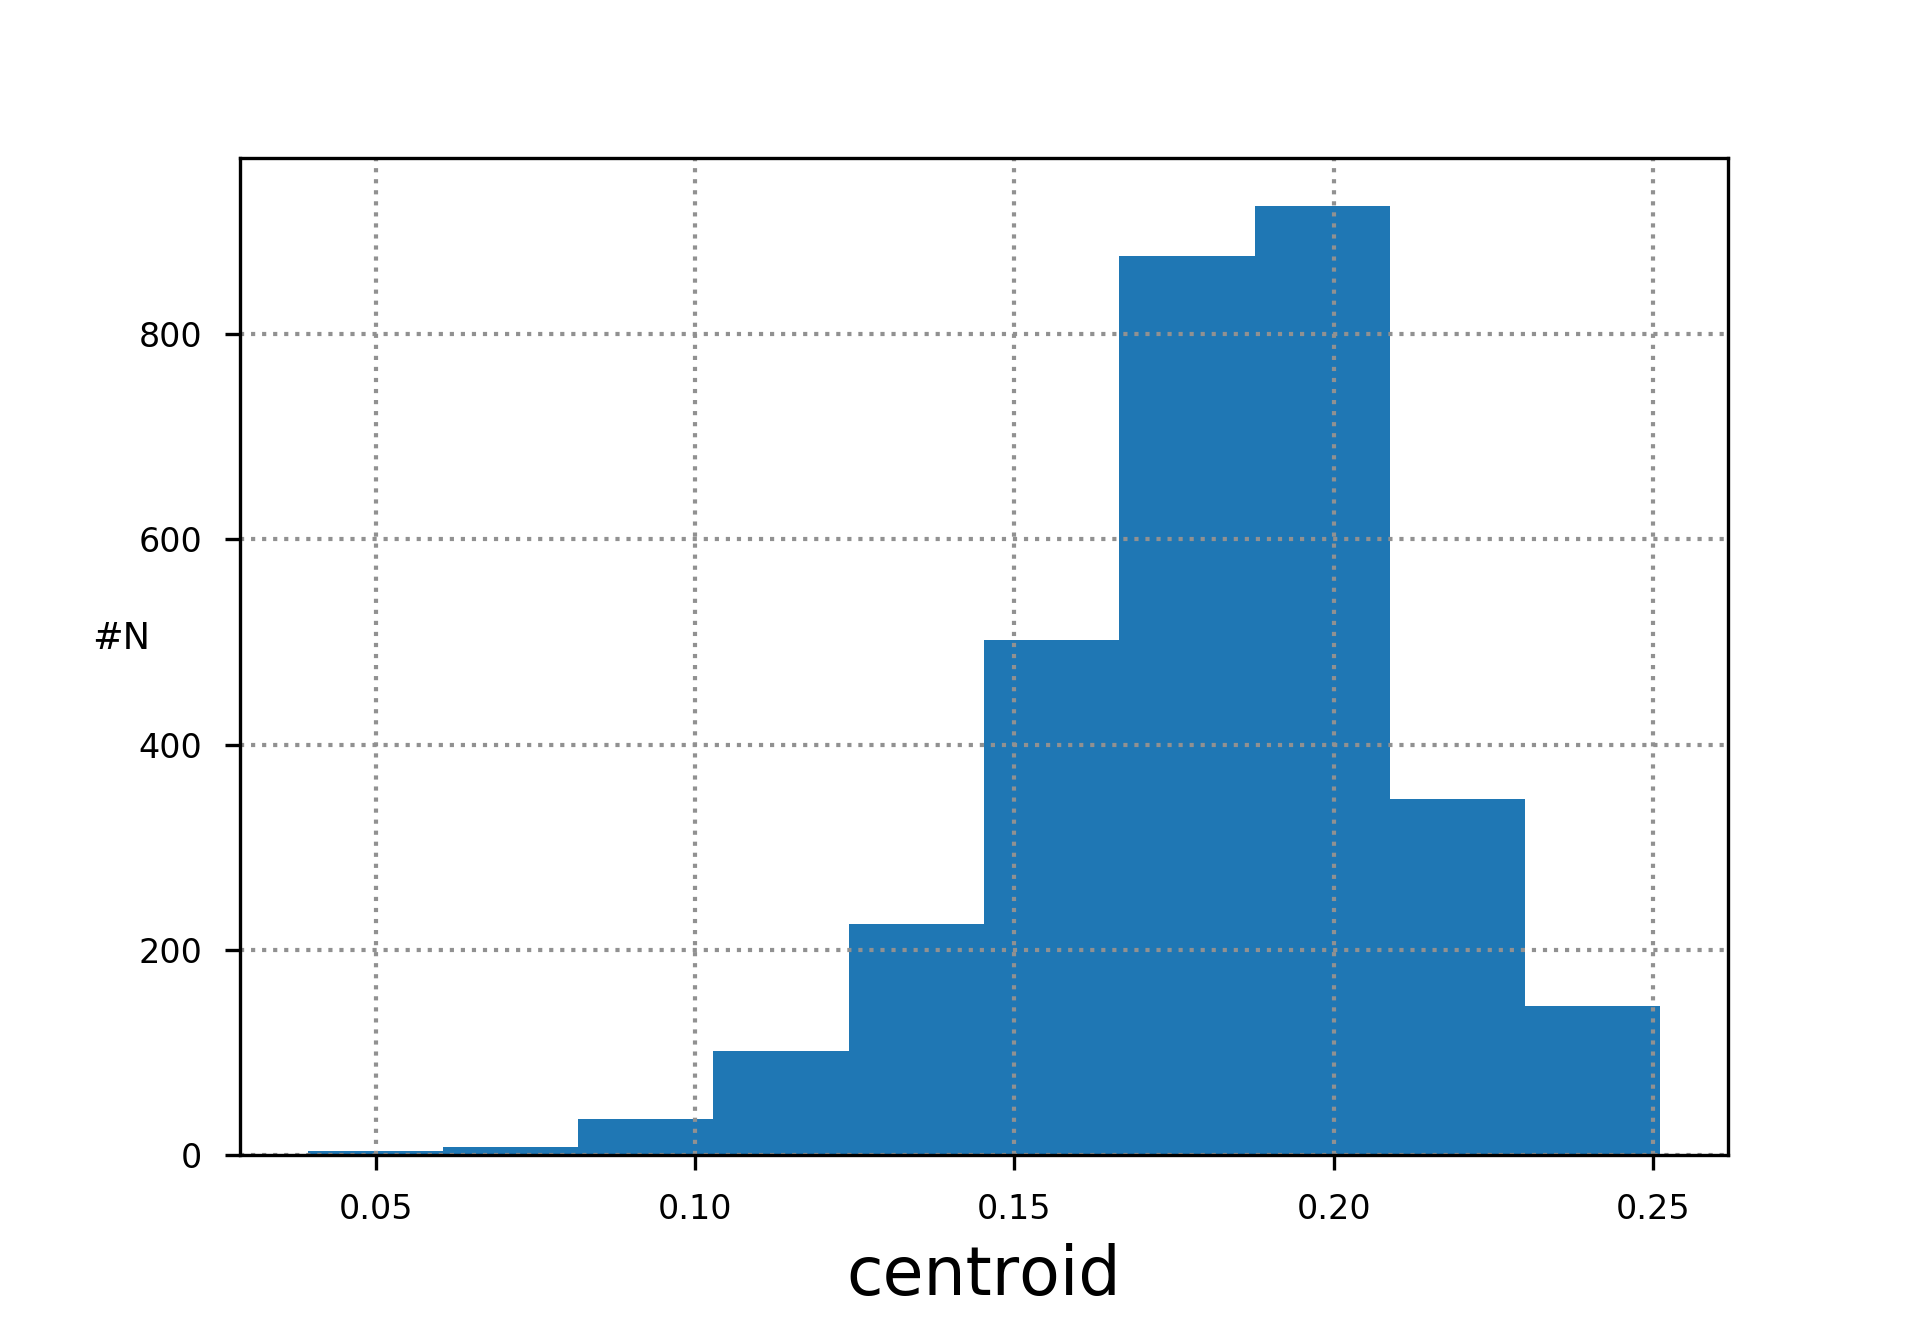
\includegraphics[width=.8\linewidth]{img1/data_histcentroid.png}
                \caption{Centroid}
            \end{subfigure}%
            \begin{subfigure}{.5\textwidth}
                \centering
                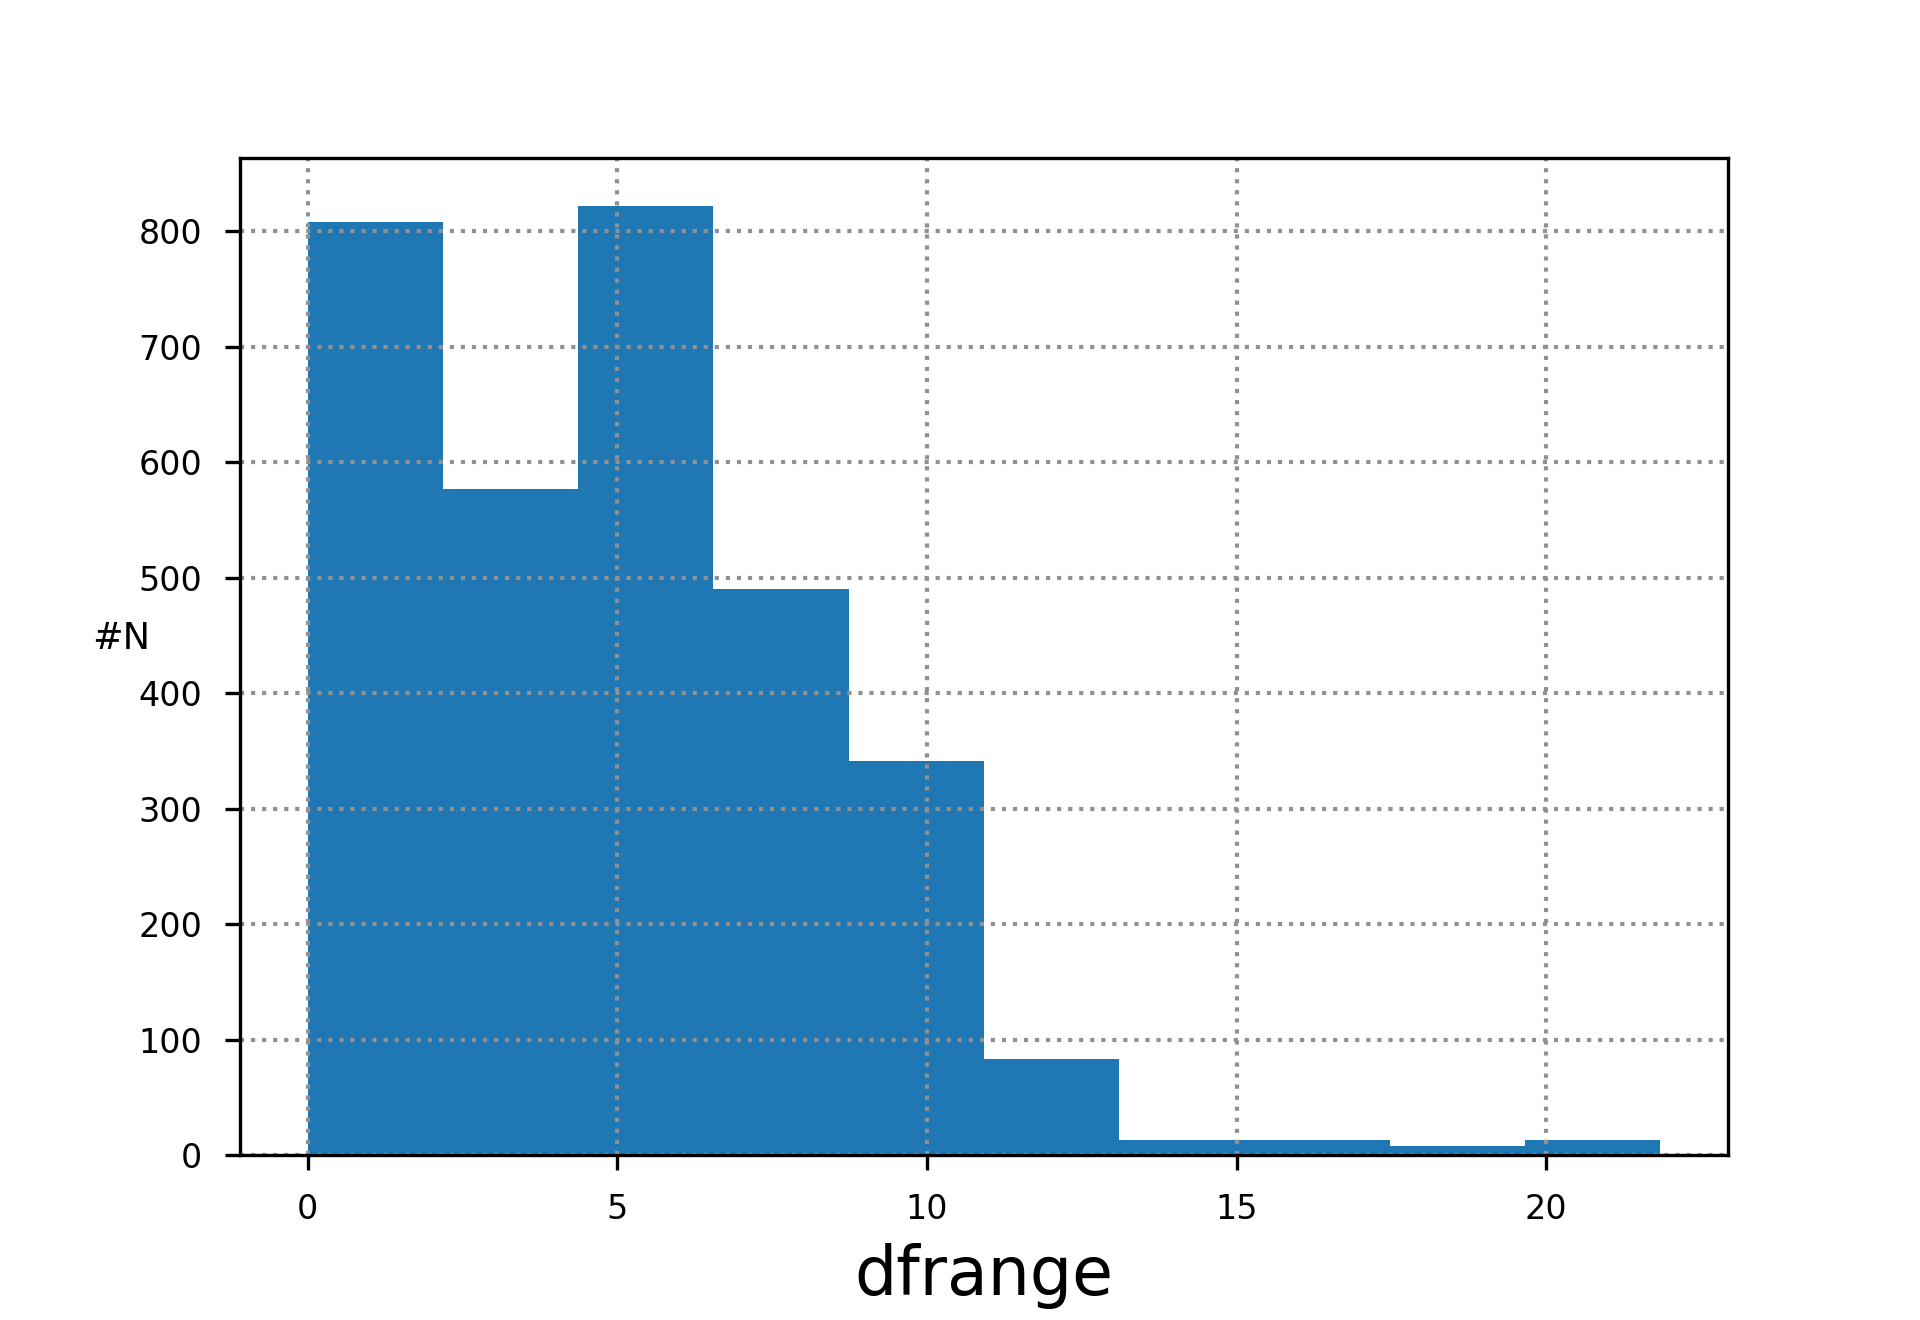
\includegraphics[width=.8\linewidth]{img1/data_histdfrange.png}
                \caption{F-Range}
            \end{subfigure}
            \begin{subfigure}{.5\textwidth}
                \centering
                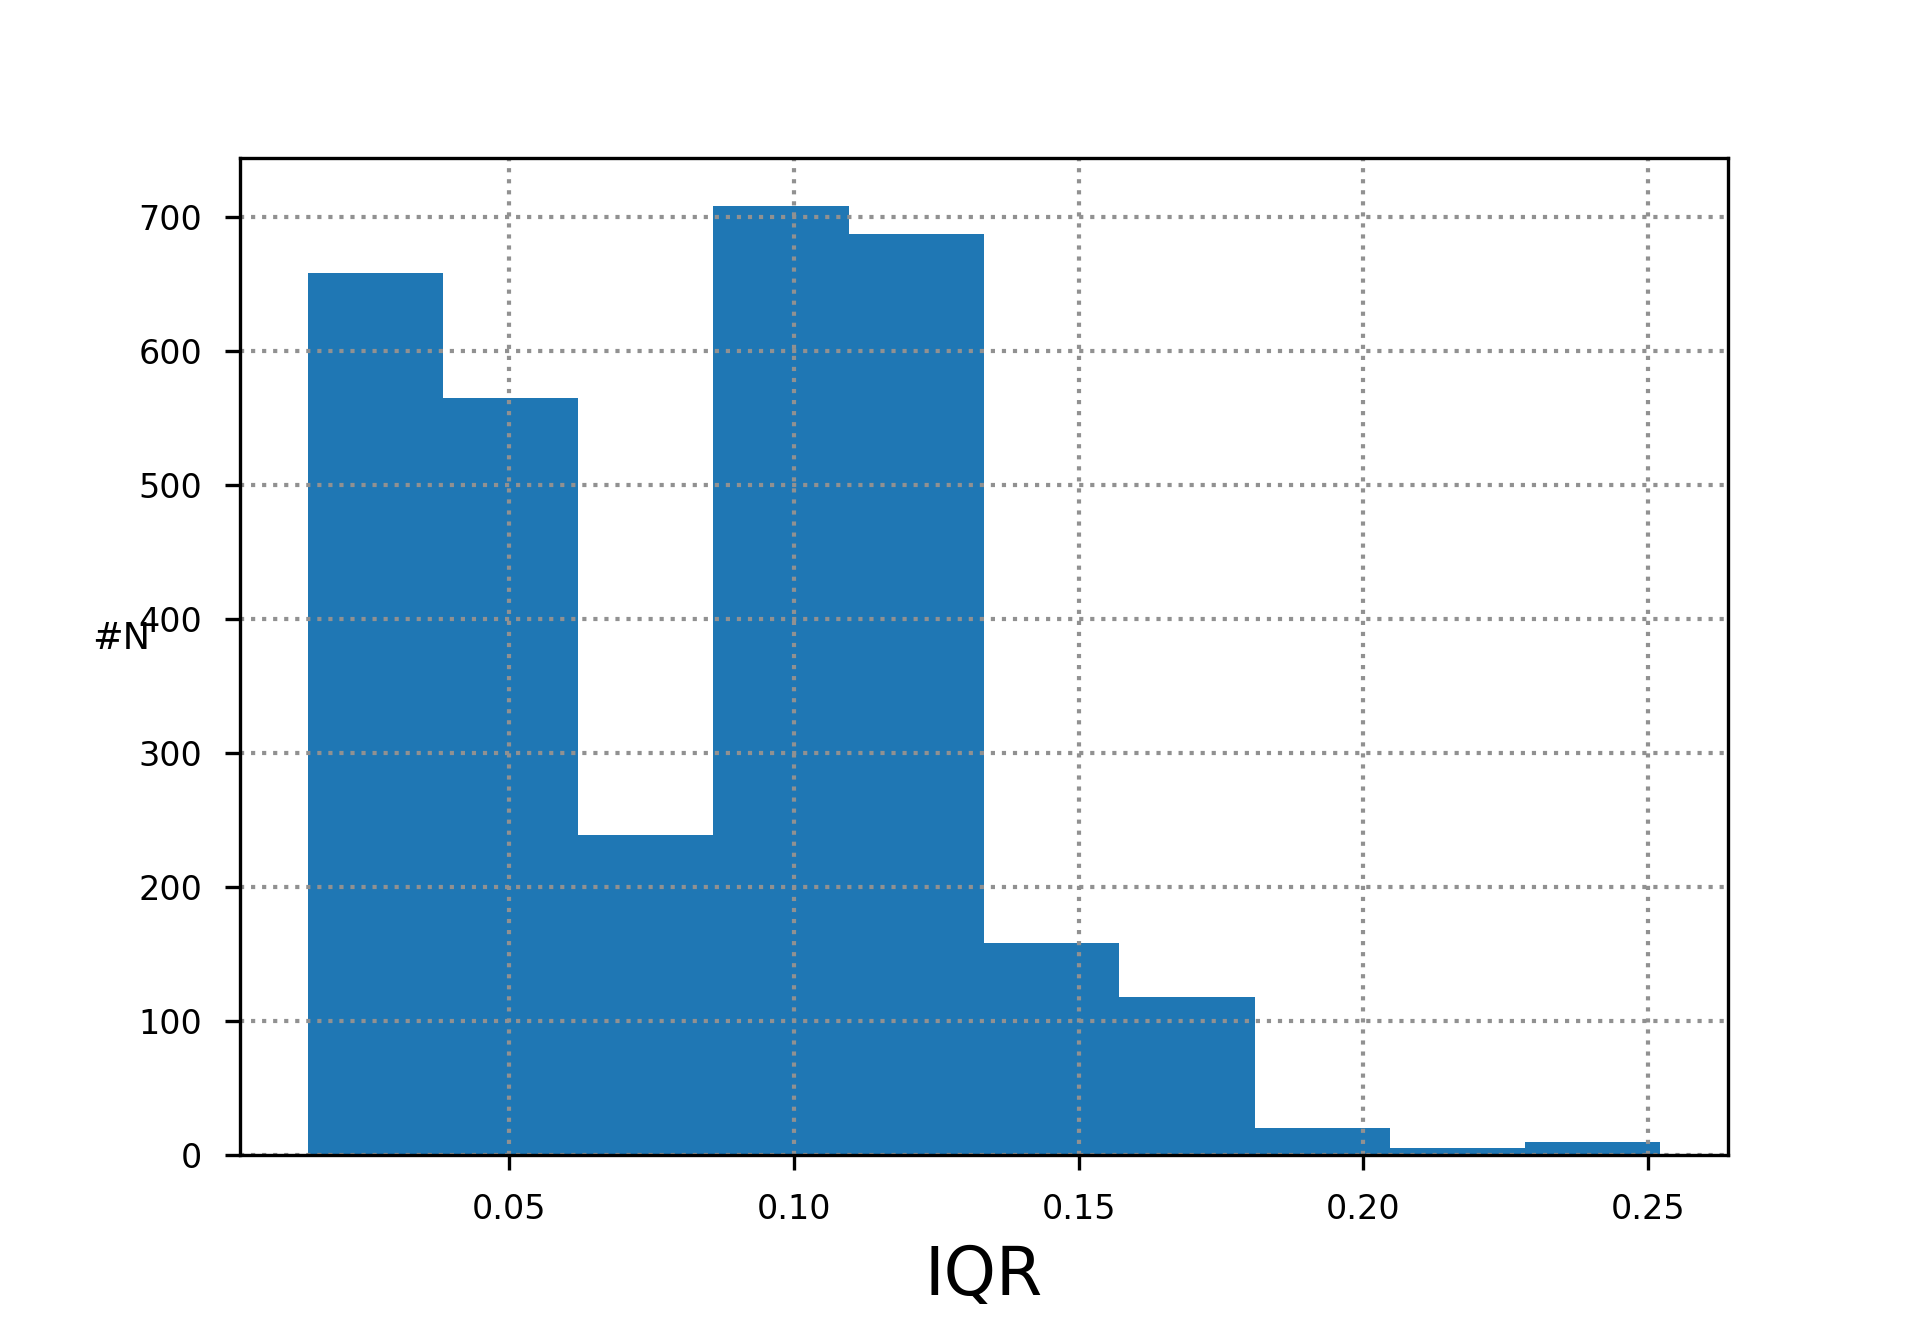
\includegraphics[width=.8\linewidth]{img1/data_histIQR.png}
                \caption{IQR}
            \end{subfigure}
            \begin{subfigure}{.5\textwidth}
                \centering
                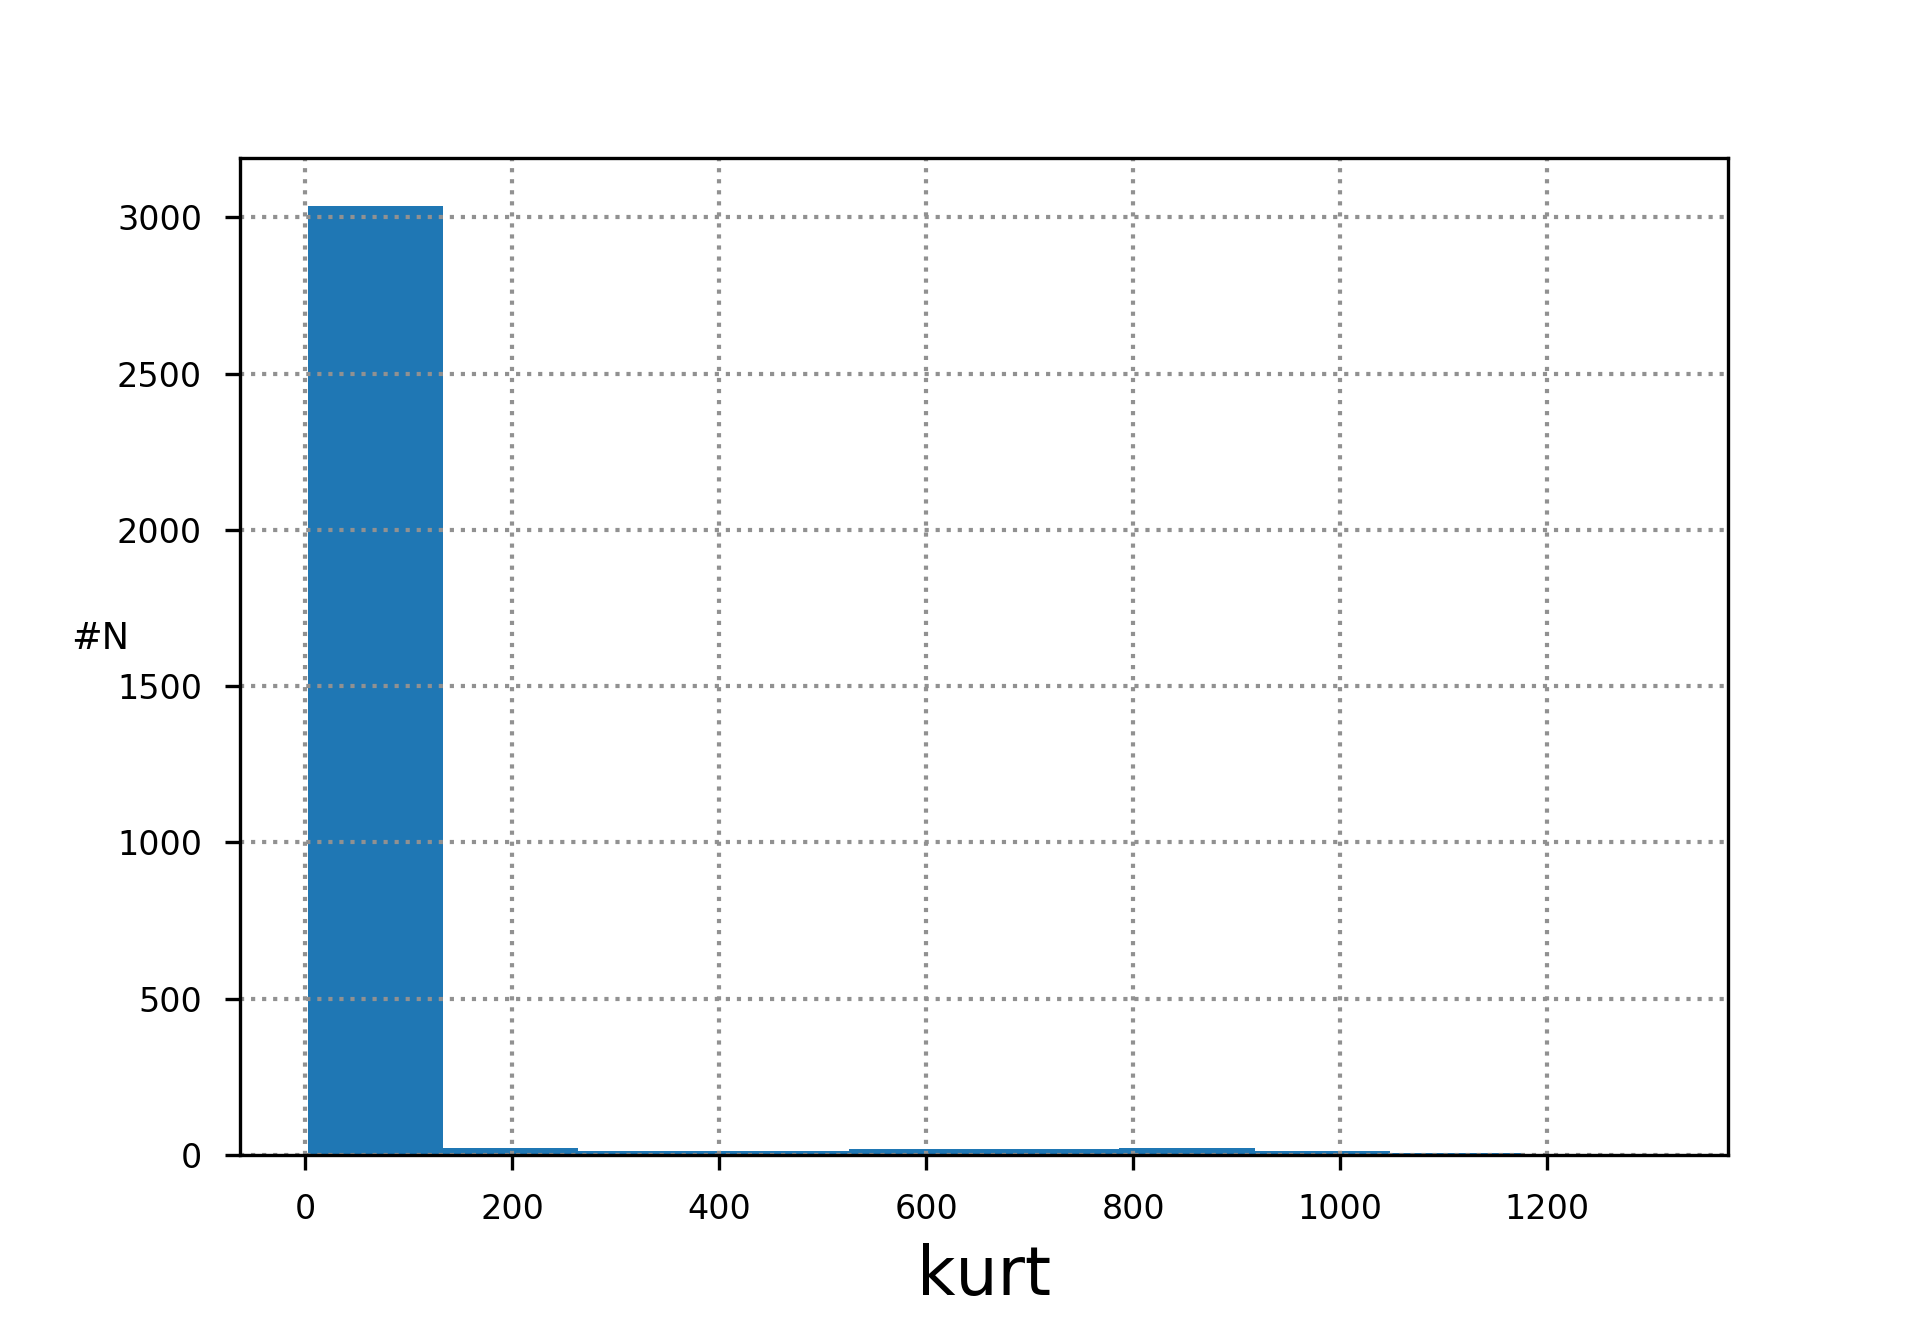
\includegraphics[width=.8\linewidth]{img1/data_histkurt.png}
                \caption{Kurt}
            \end{subfigure}
            \begin{subfigure}{.5\textwidth}
                \centering
                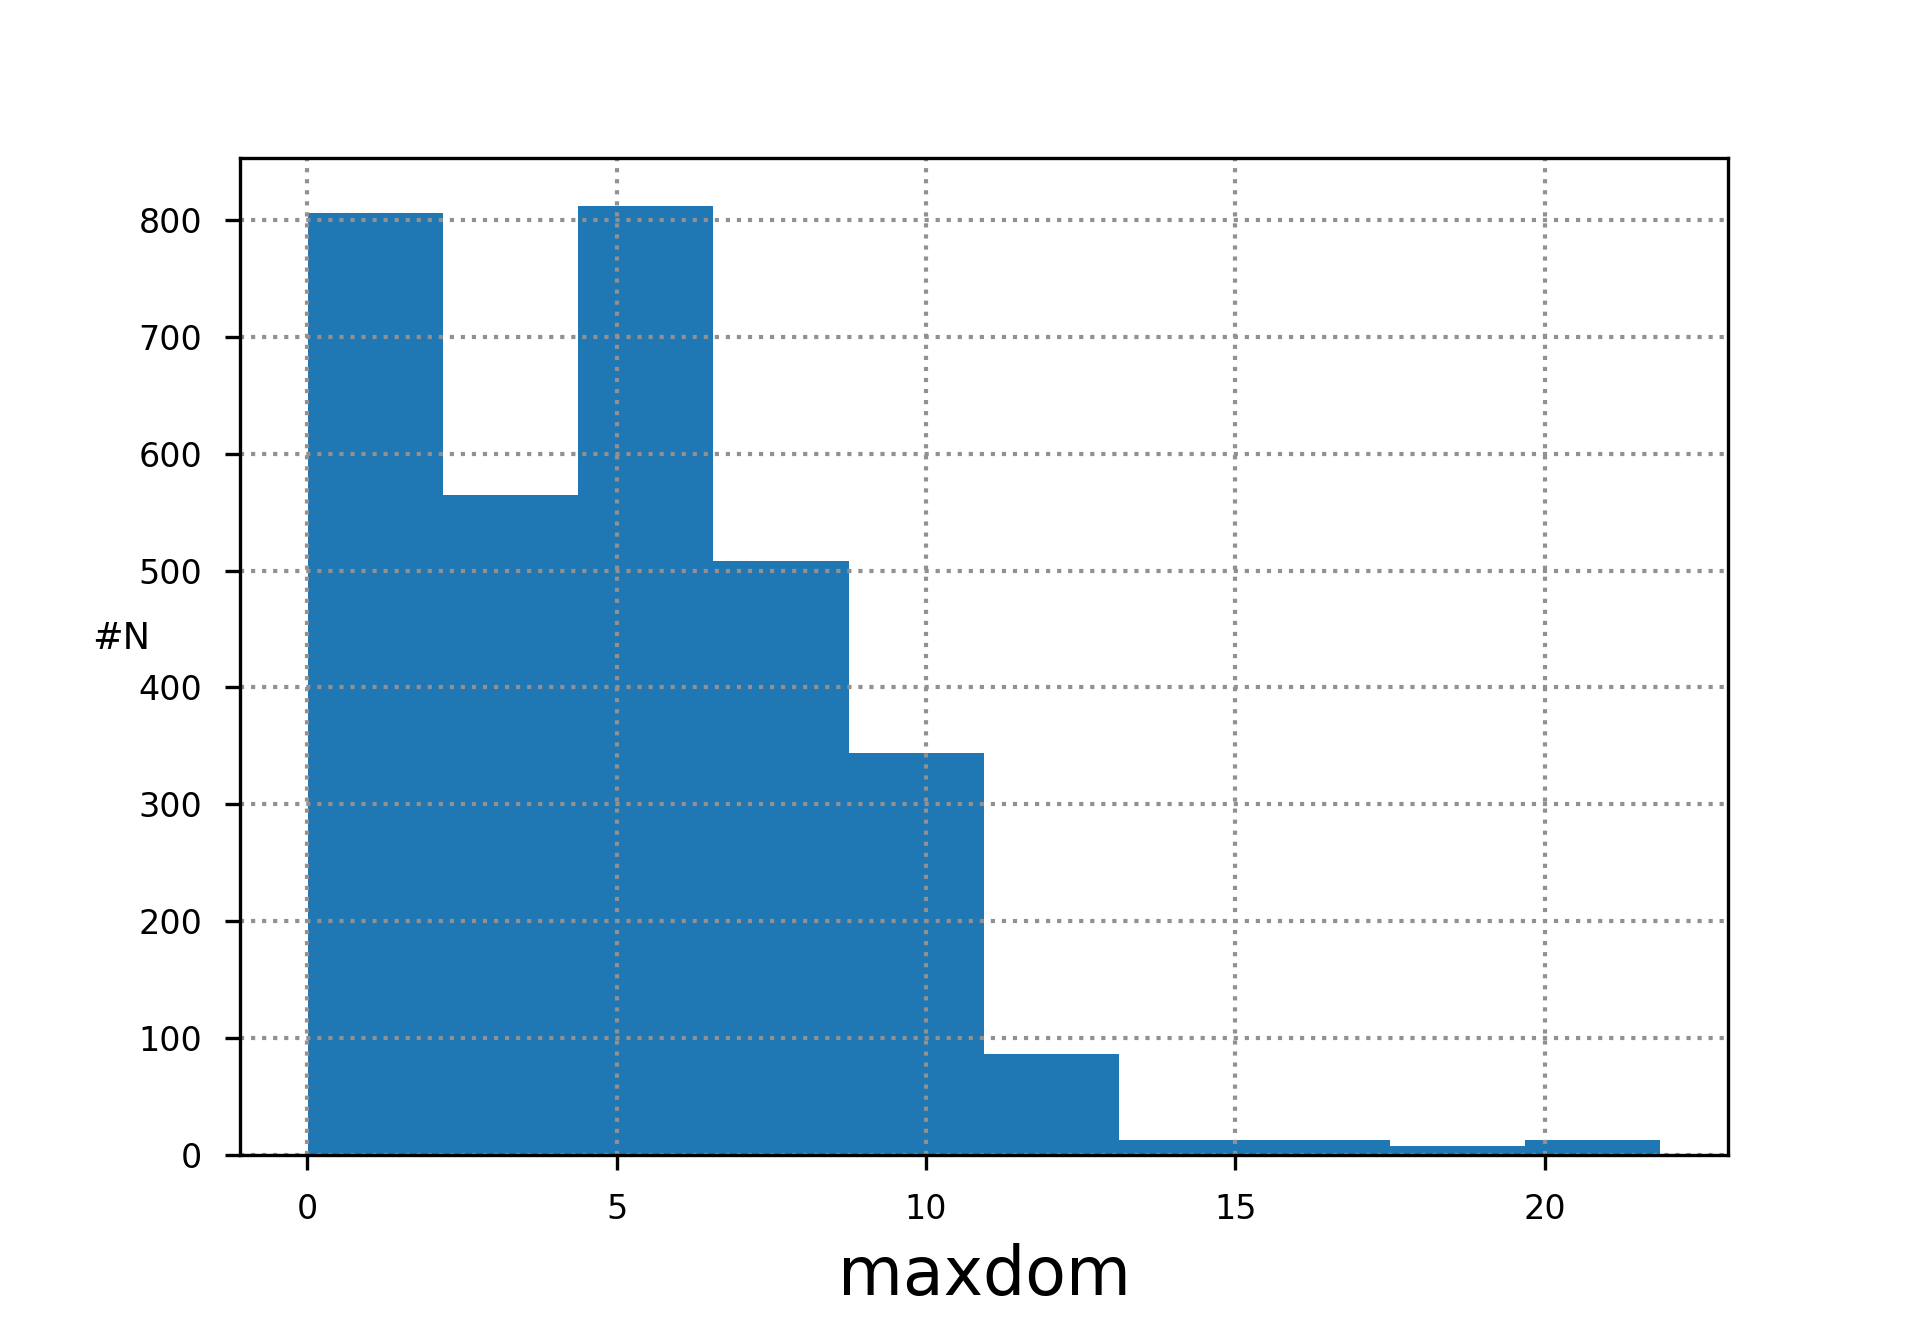
\includegraphics[width=.8\linewidth]{img1/data_histmaxdom.png}
                \caption{Max dom}
            \end{subfigure}
            \begin{subfigure}{.5\textwidth}
                \centering
                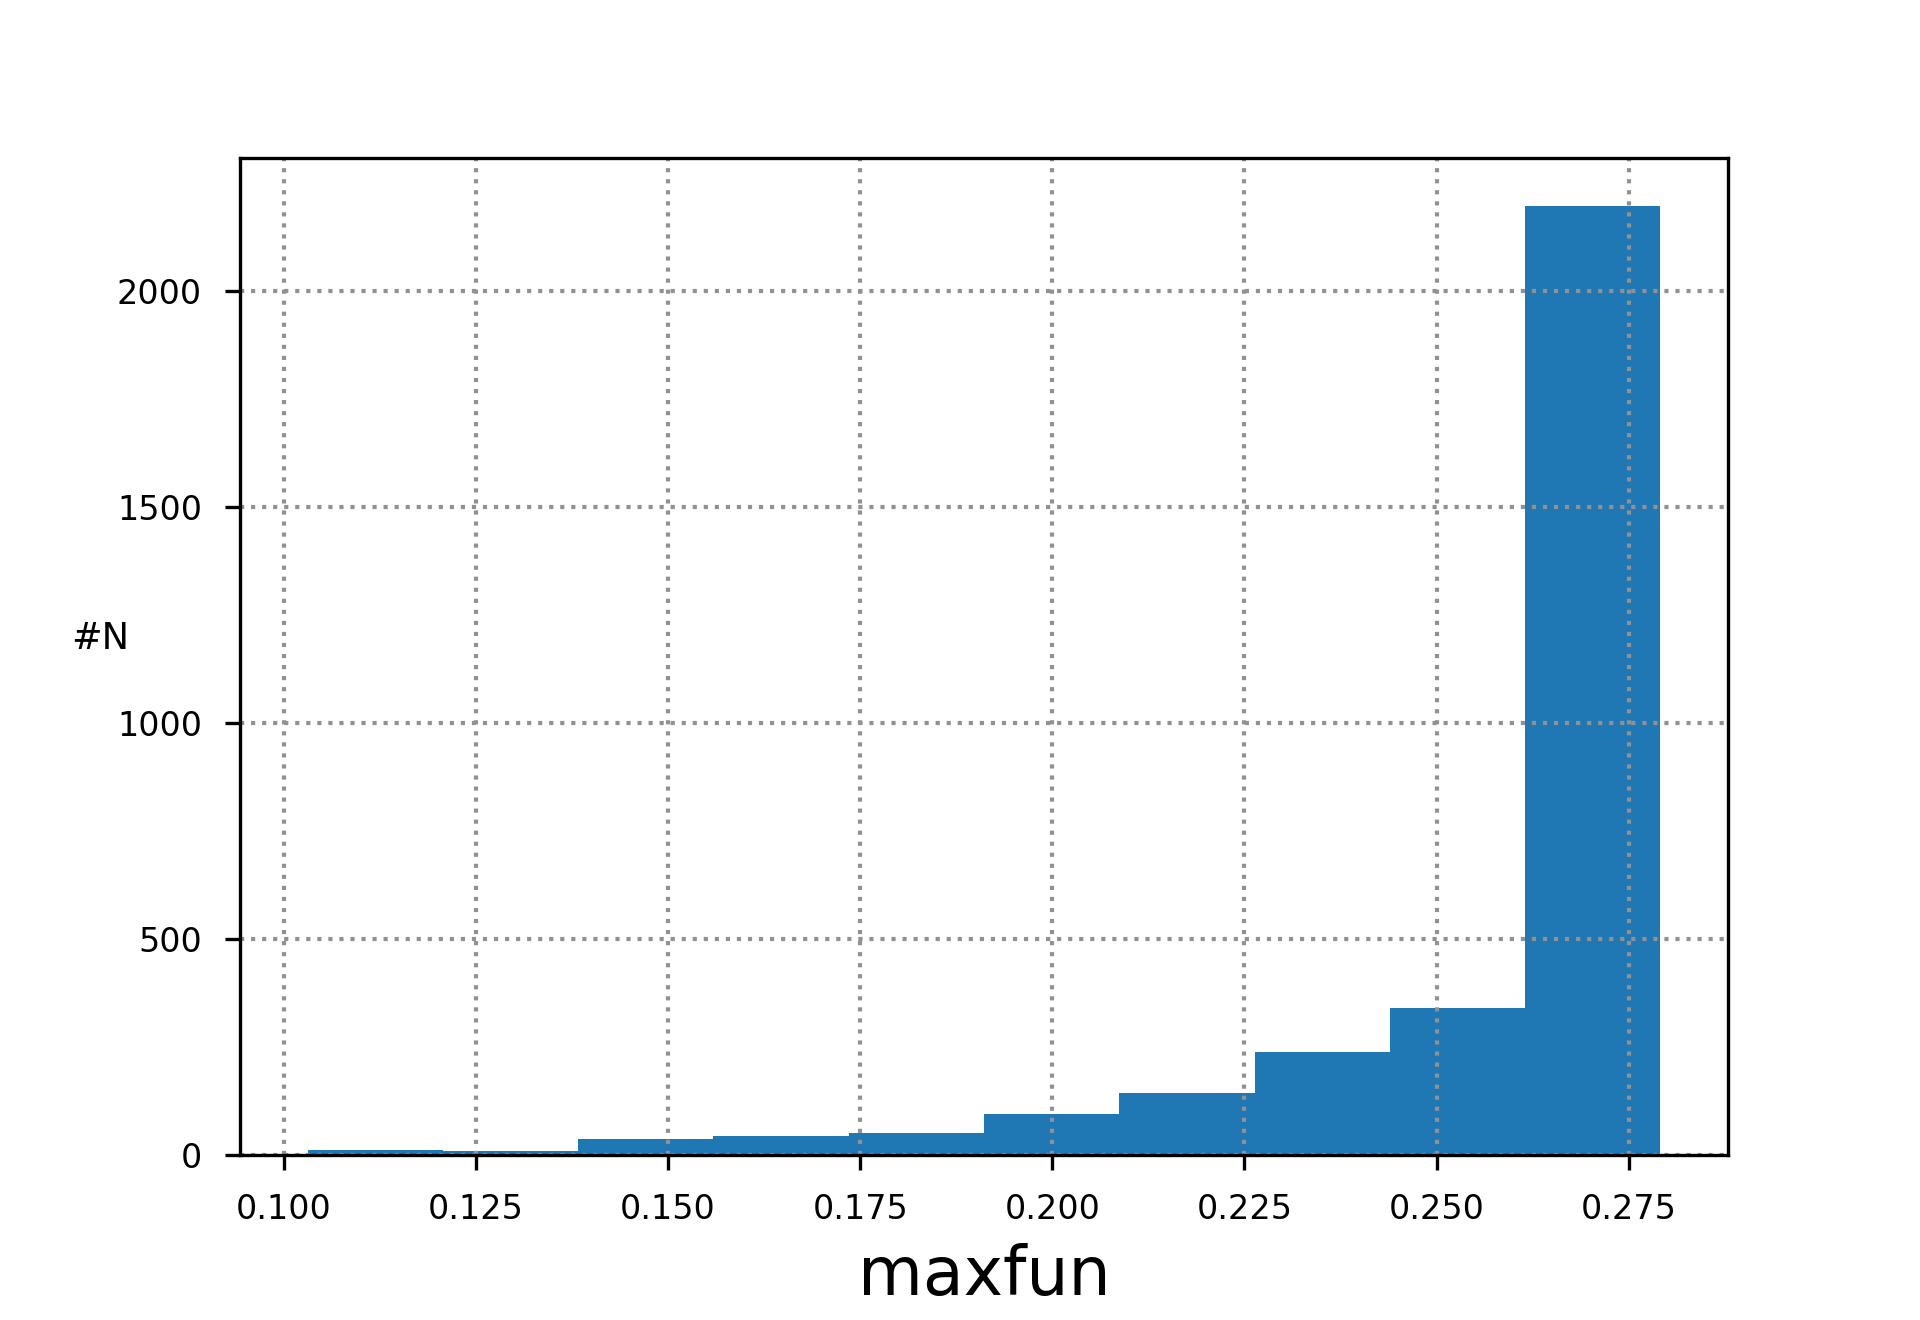
\includegraphics[width=.8\linewidth]{img1/data_histmaxfun.png}
                \caption{Max fun}
            \end{subfigure}
            \begin{subfigure}{.5\textwidth}
                \centering
                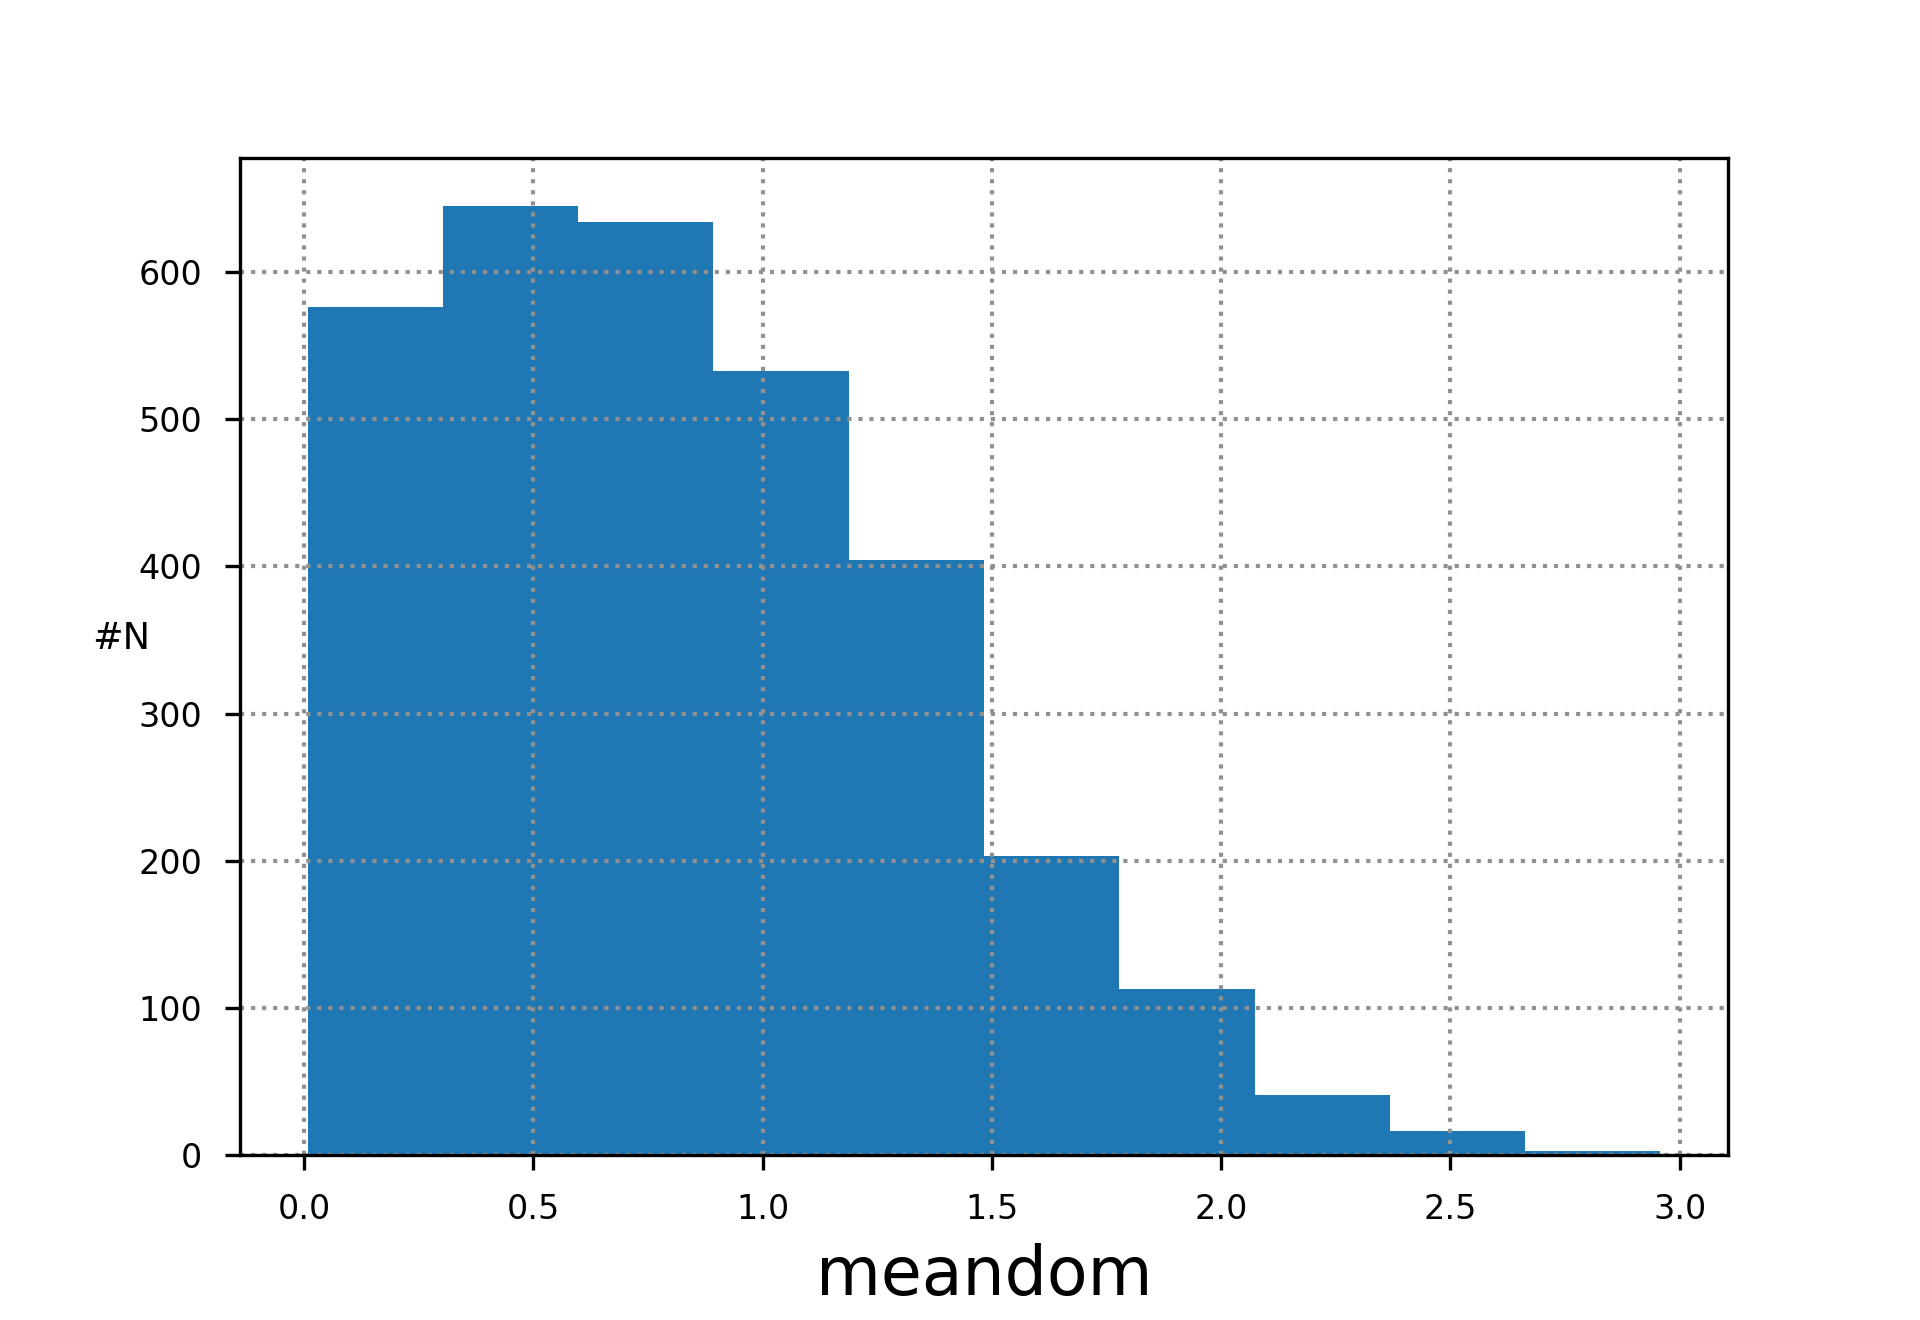
\includegraphics[width=.8\linewidth]{img1/data_histmeandom.png}
                \caption{Mean dom}
            \end{subfigure}
            \begin{subfigure}{.5\textwidth}
                \centering
                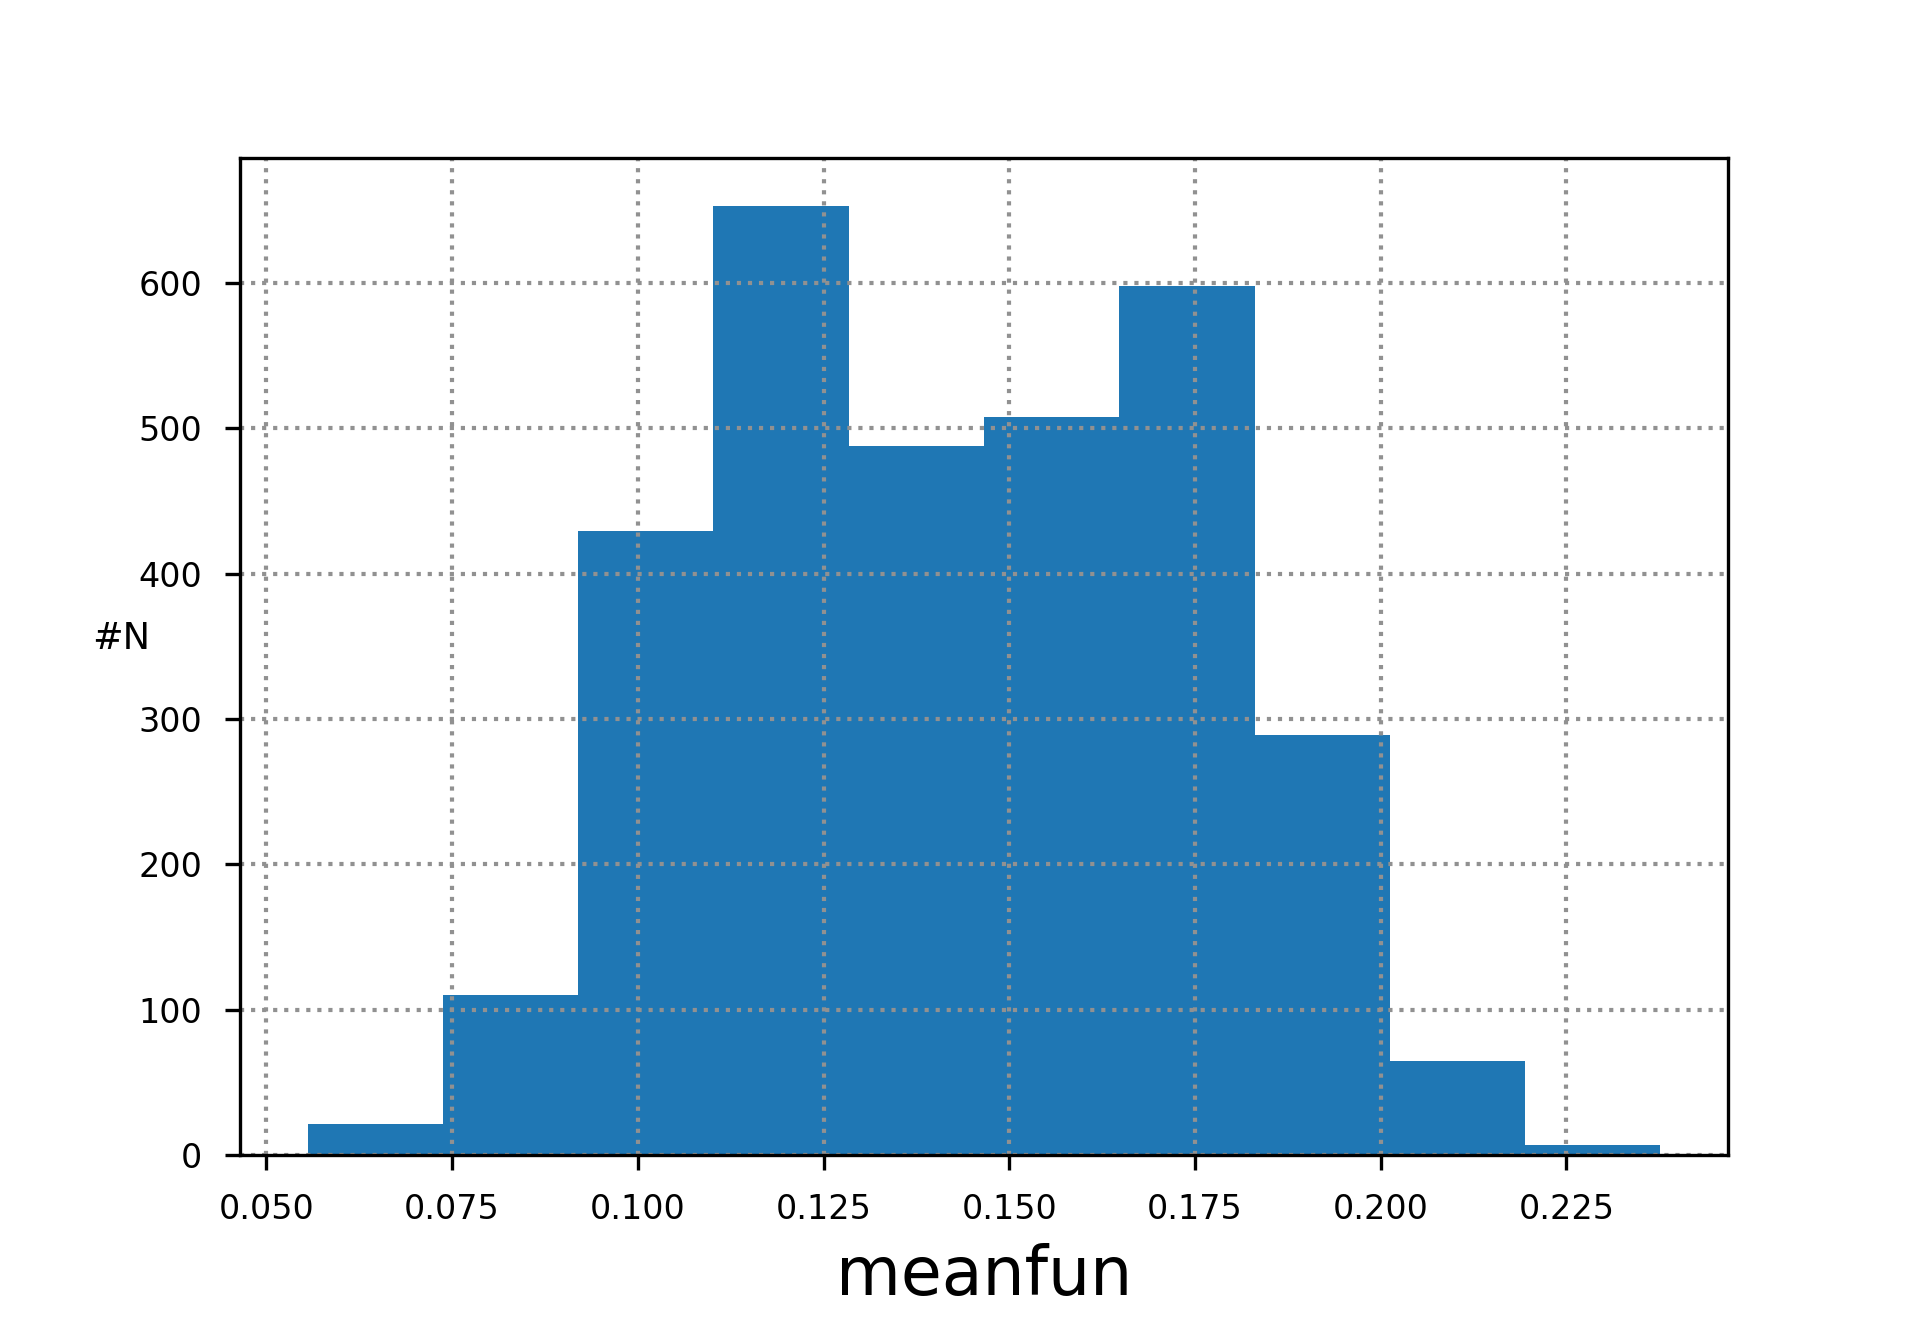
\includegraphics[width=.8\linewidth]{img1/data_histmeanfun.png}
                \caption{Mean fun}
            \end{subfigure}
        \caption{Classificação binária: Histograma dos atributos (1)}
        \label{fig:a_hist_1}
        \end{figure}
        \begin{figure}[H]
            \begin{subfigure}{.5\textwidth}
                \centering
                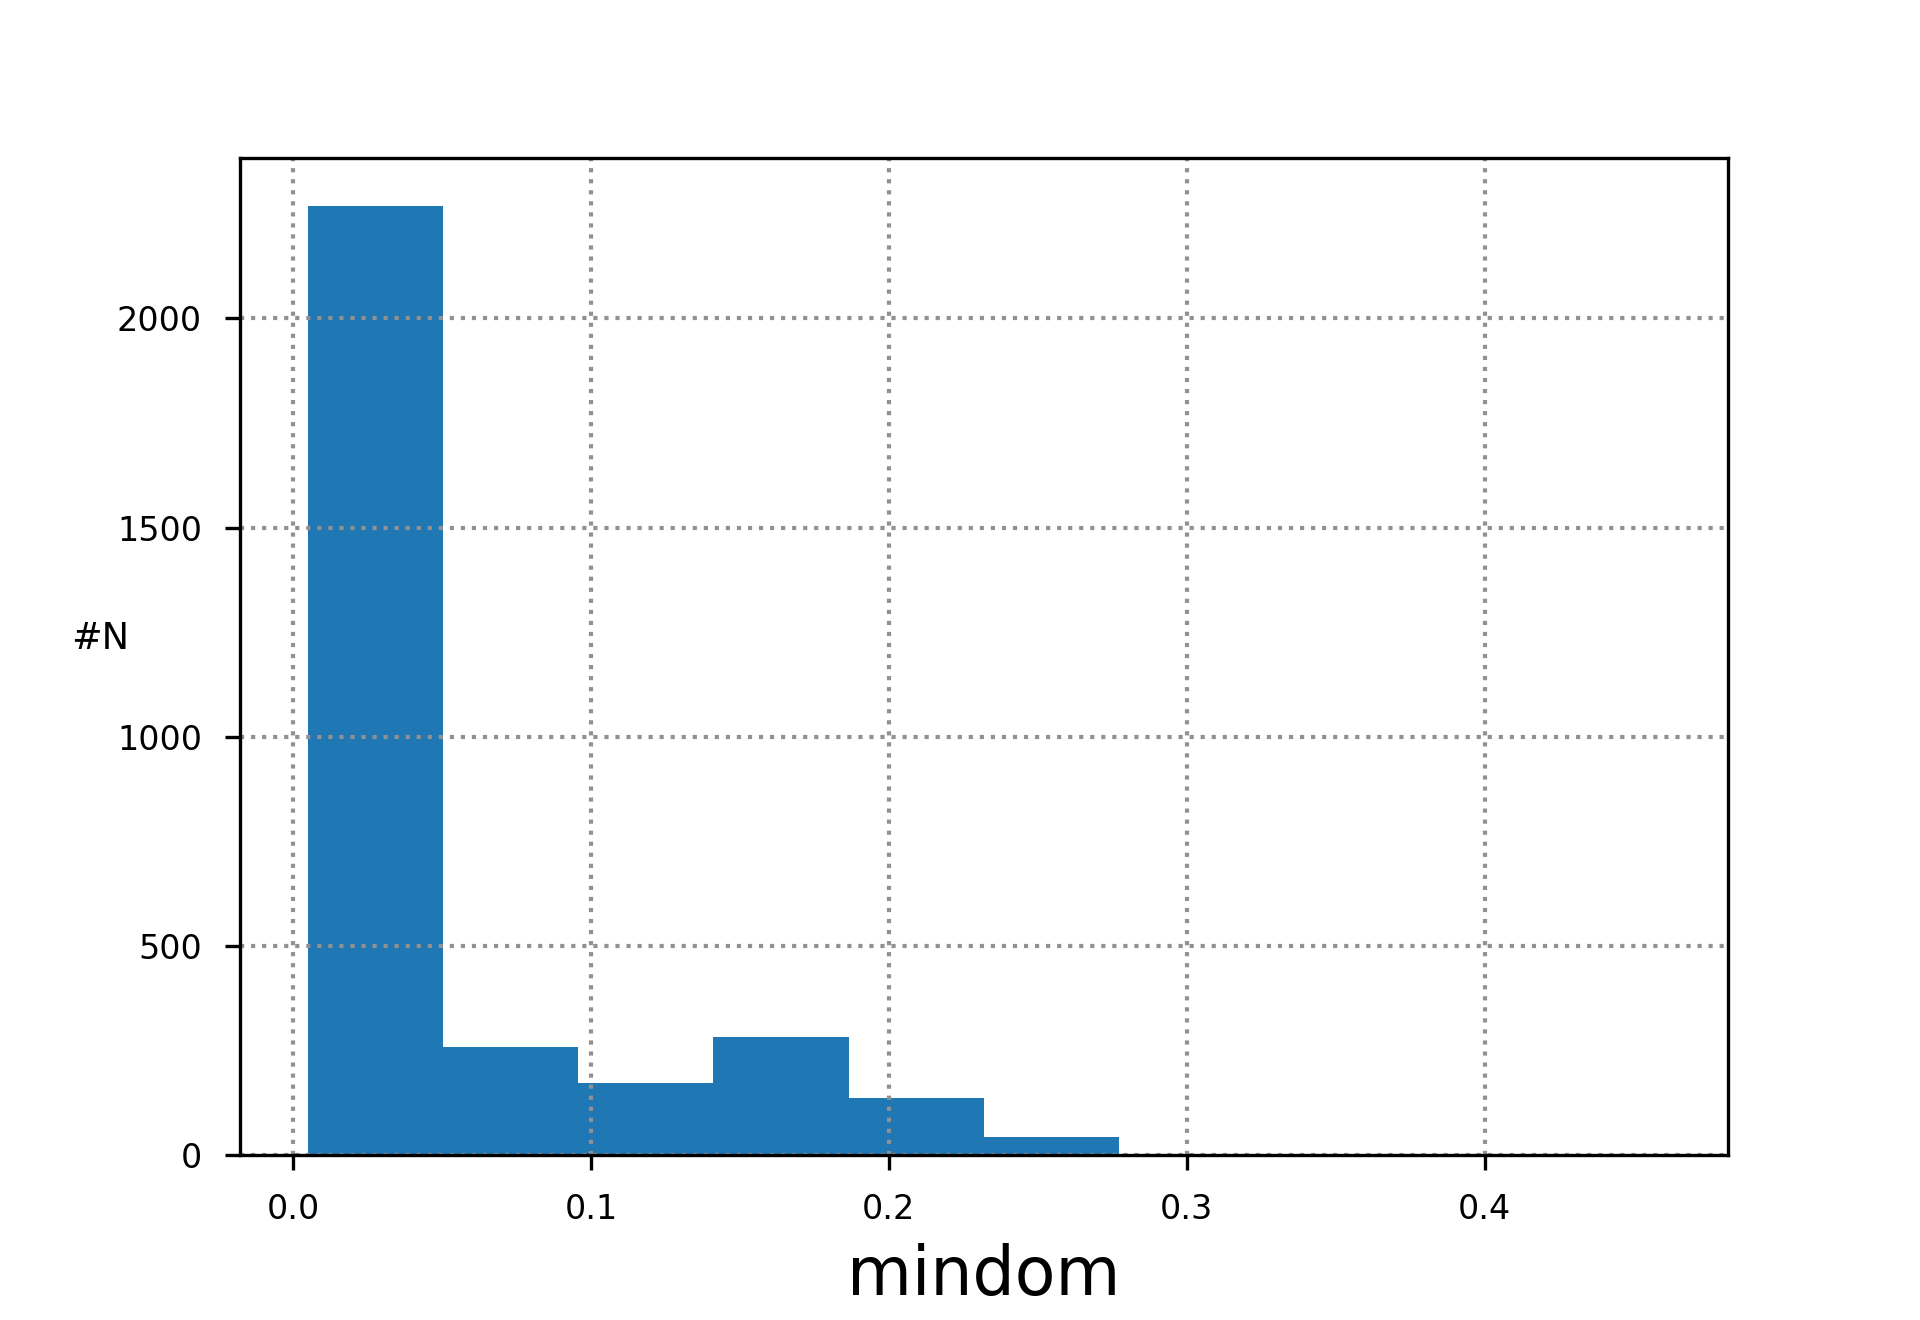
\includegraphics[width=.8\linewidth]{img1/data_histmindom.png}
                \caption{Min dom}
            \end{subfigure}
            \begin{subfigure}{.5\textwidth}
                \centering
                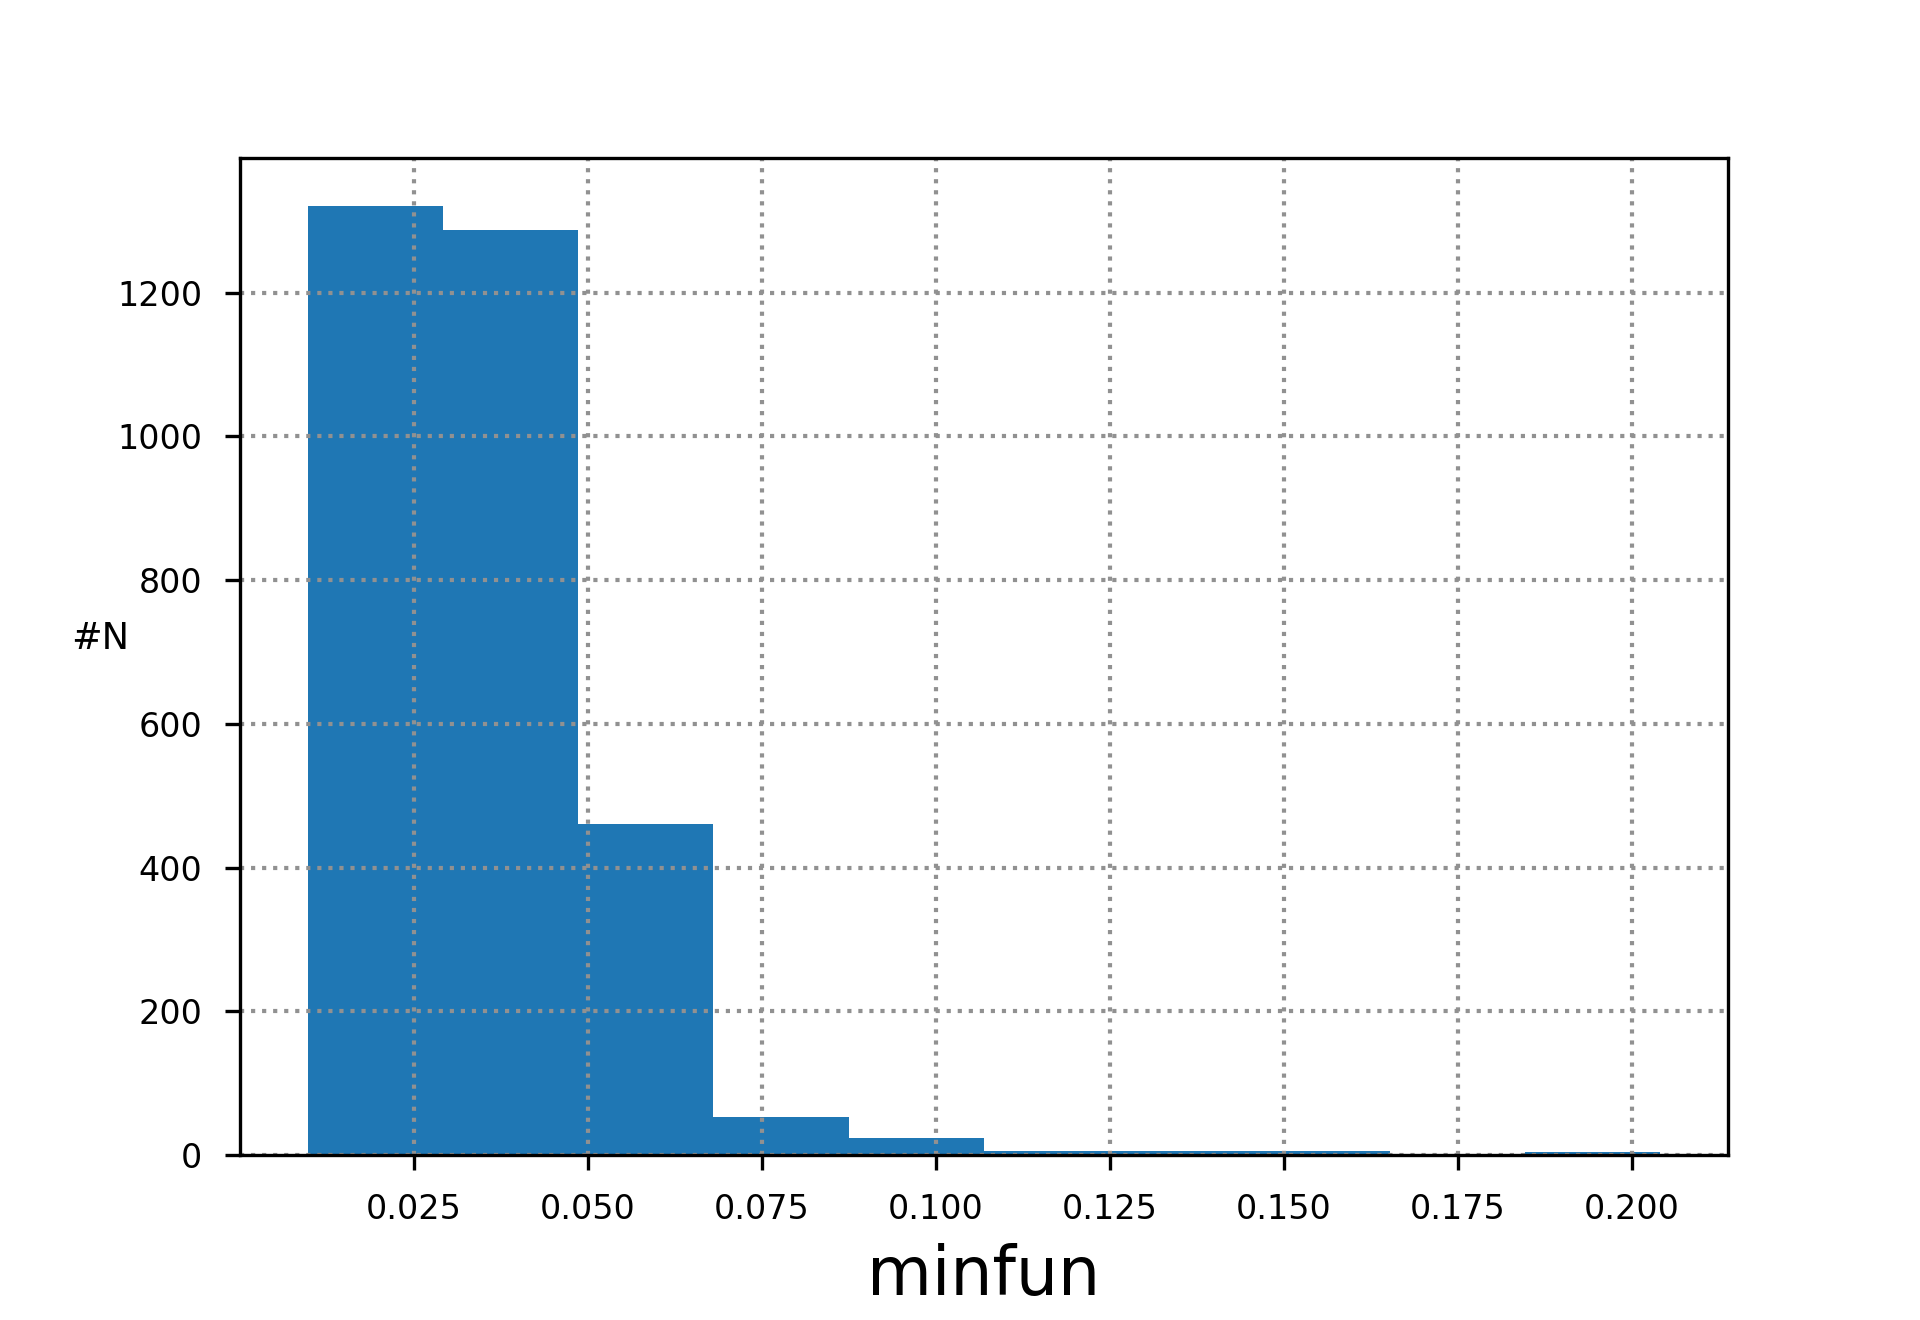
\includegraphics[width=.8\linewidth]{img1/data_histminfun.png}
                \caption{Min fun}
            \end{subfigure}
            \begin{subfigure}{.5\textwidth}
                \centering
                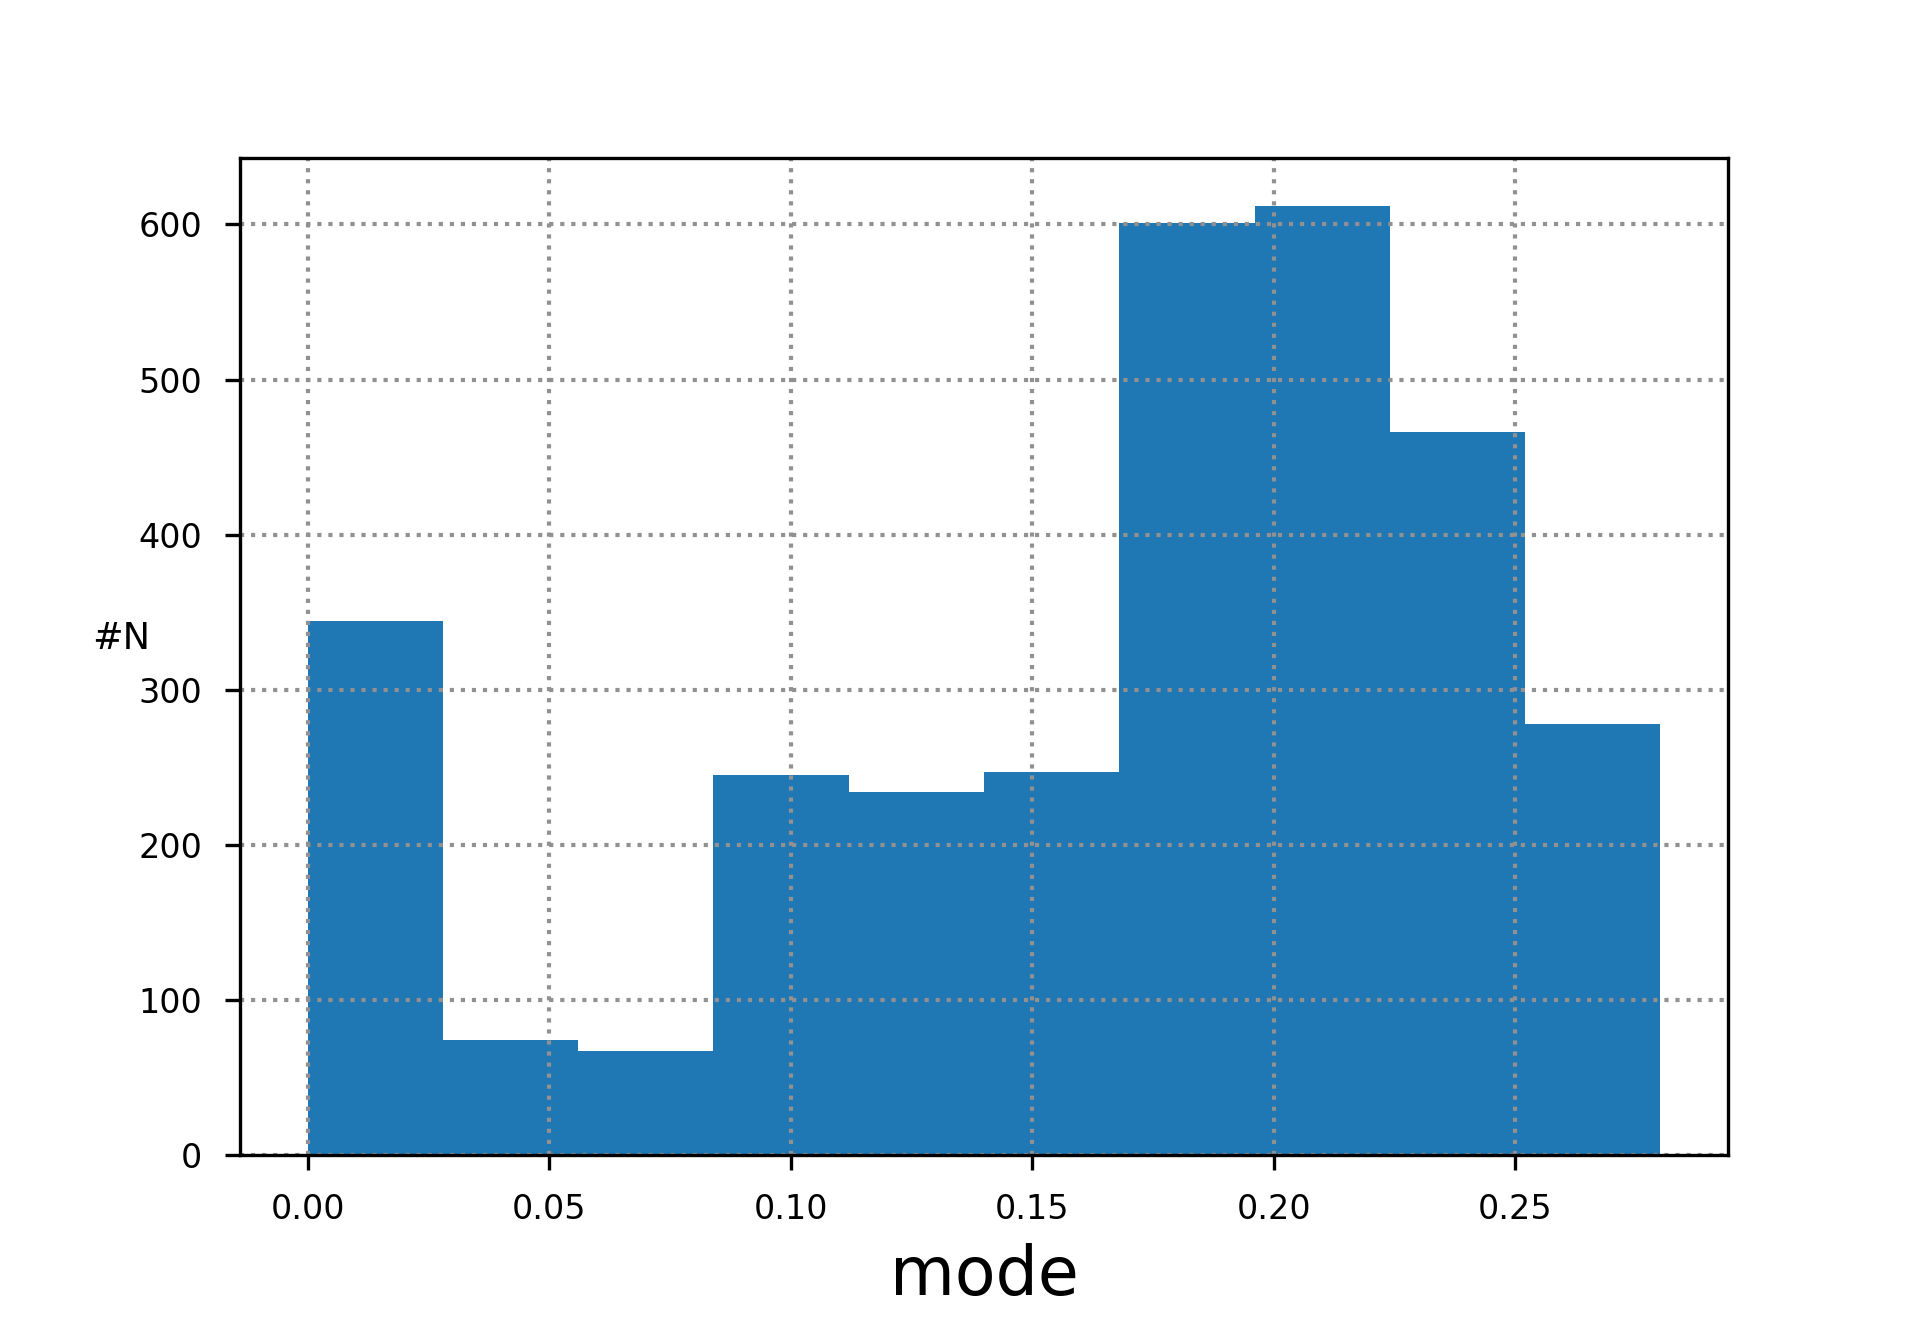
\includegraphics[width=.8\linewidth]{img1/data_histmode.png}
                \caption{Mode}
            \end{subfigure}
            \begin{subfigure}{.5\textwidth}
                \centering
                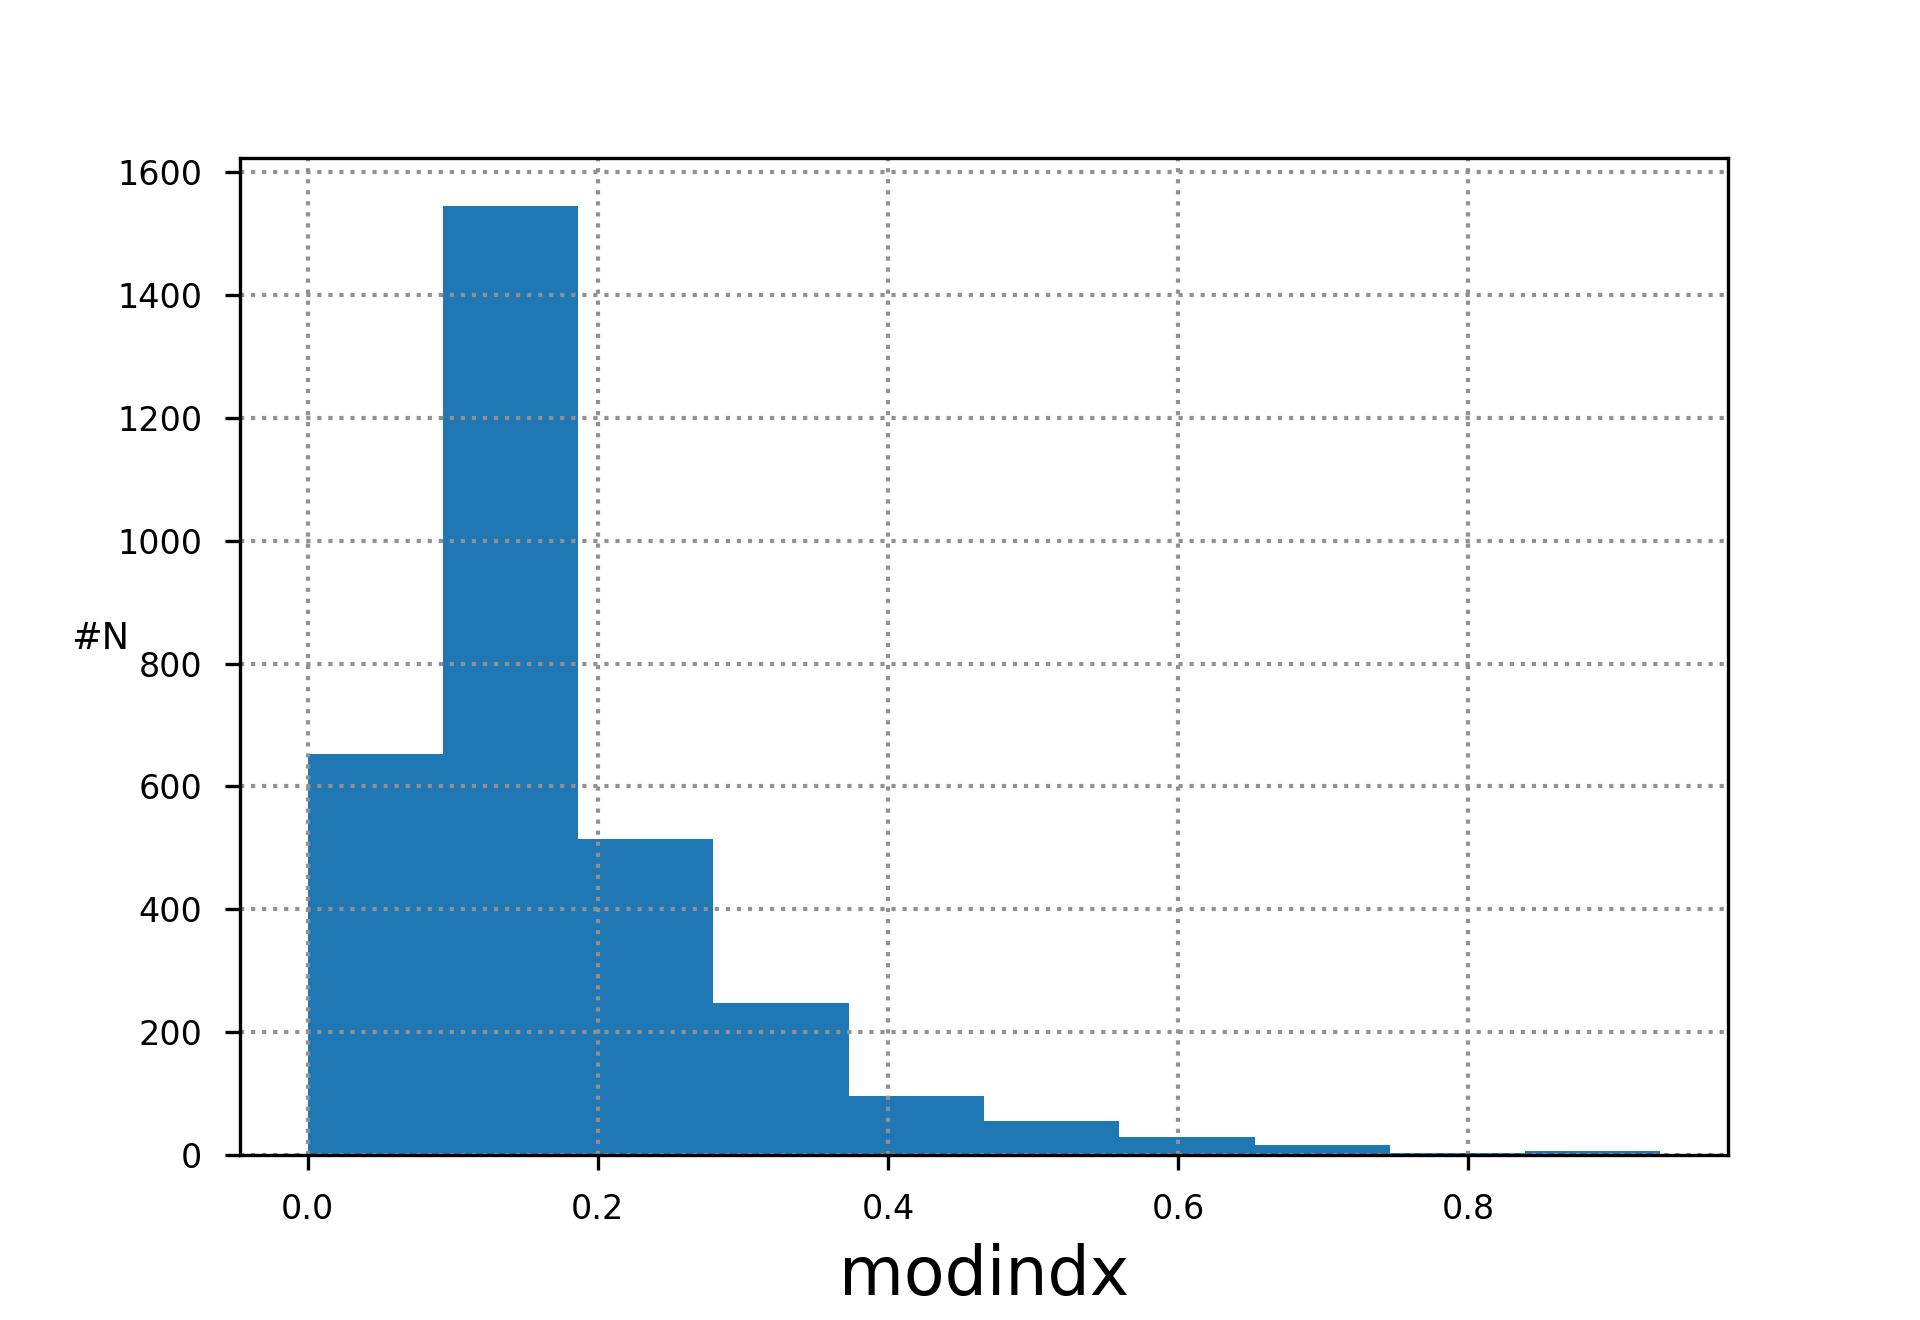
\includegraphics[width=.8\linewidth]{img1/data_histmodindx.png}
                \caption{modindx}
            \end{subfigure}
            \begin{subfigure}{.5\textwidth}
                \centering
                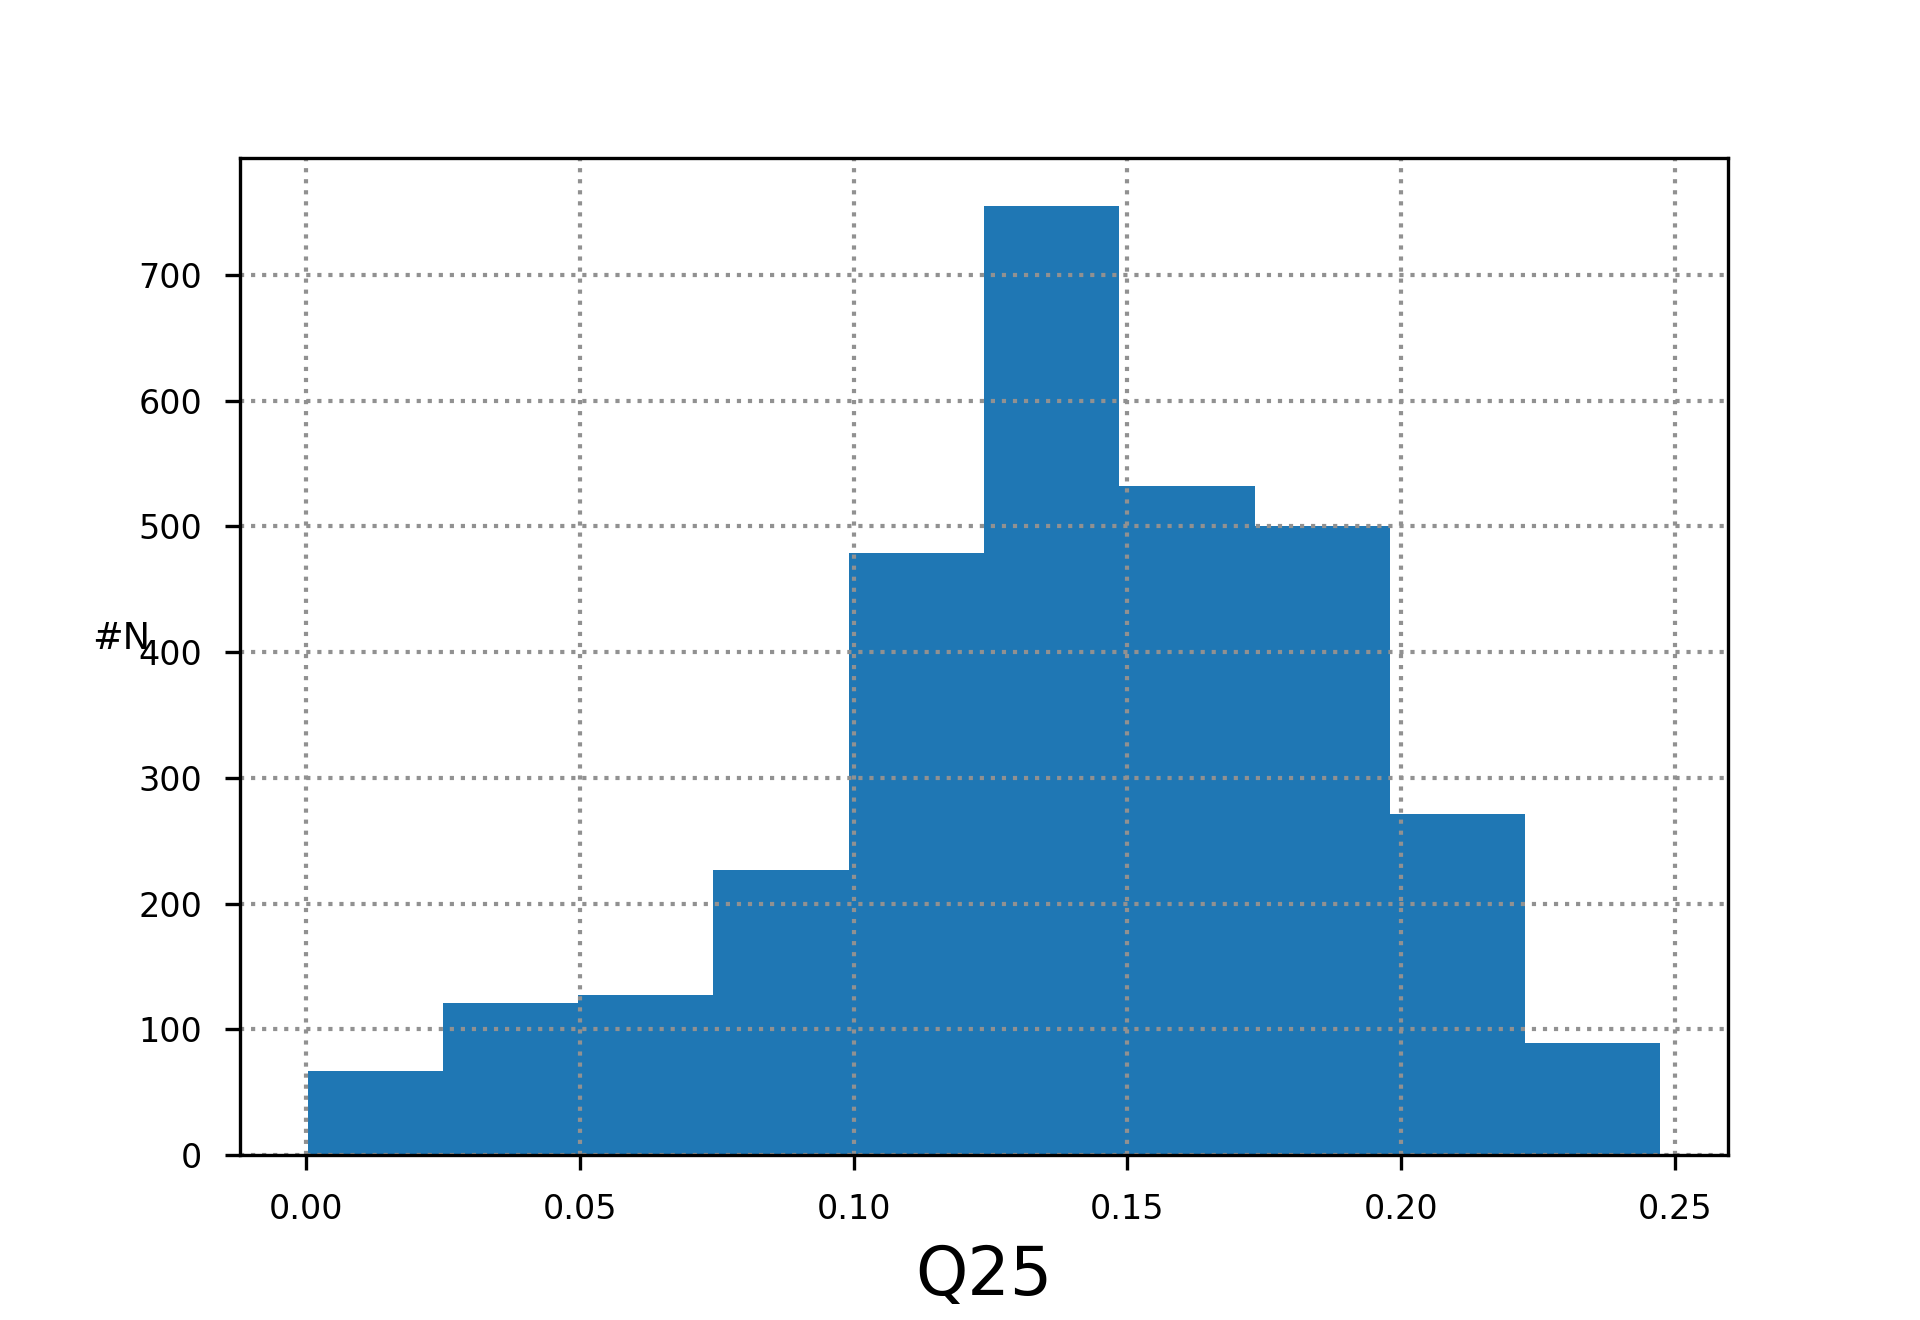
\includegraphics[width=.8\linewidth]{img1/data_histQ25.png}
                \caption{Q25}
            \end{subfigure}
            \begin{subfigure}{.5\textwidth}
                \centering
                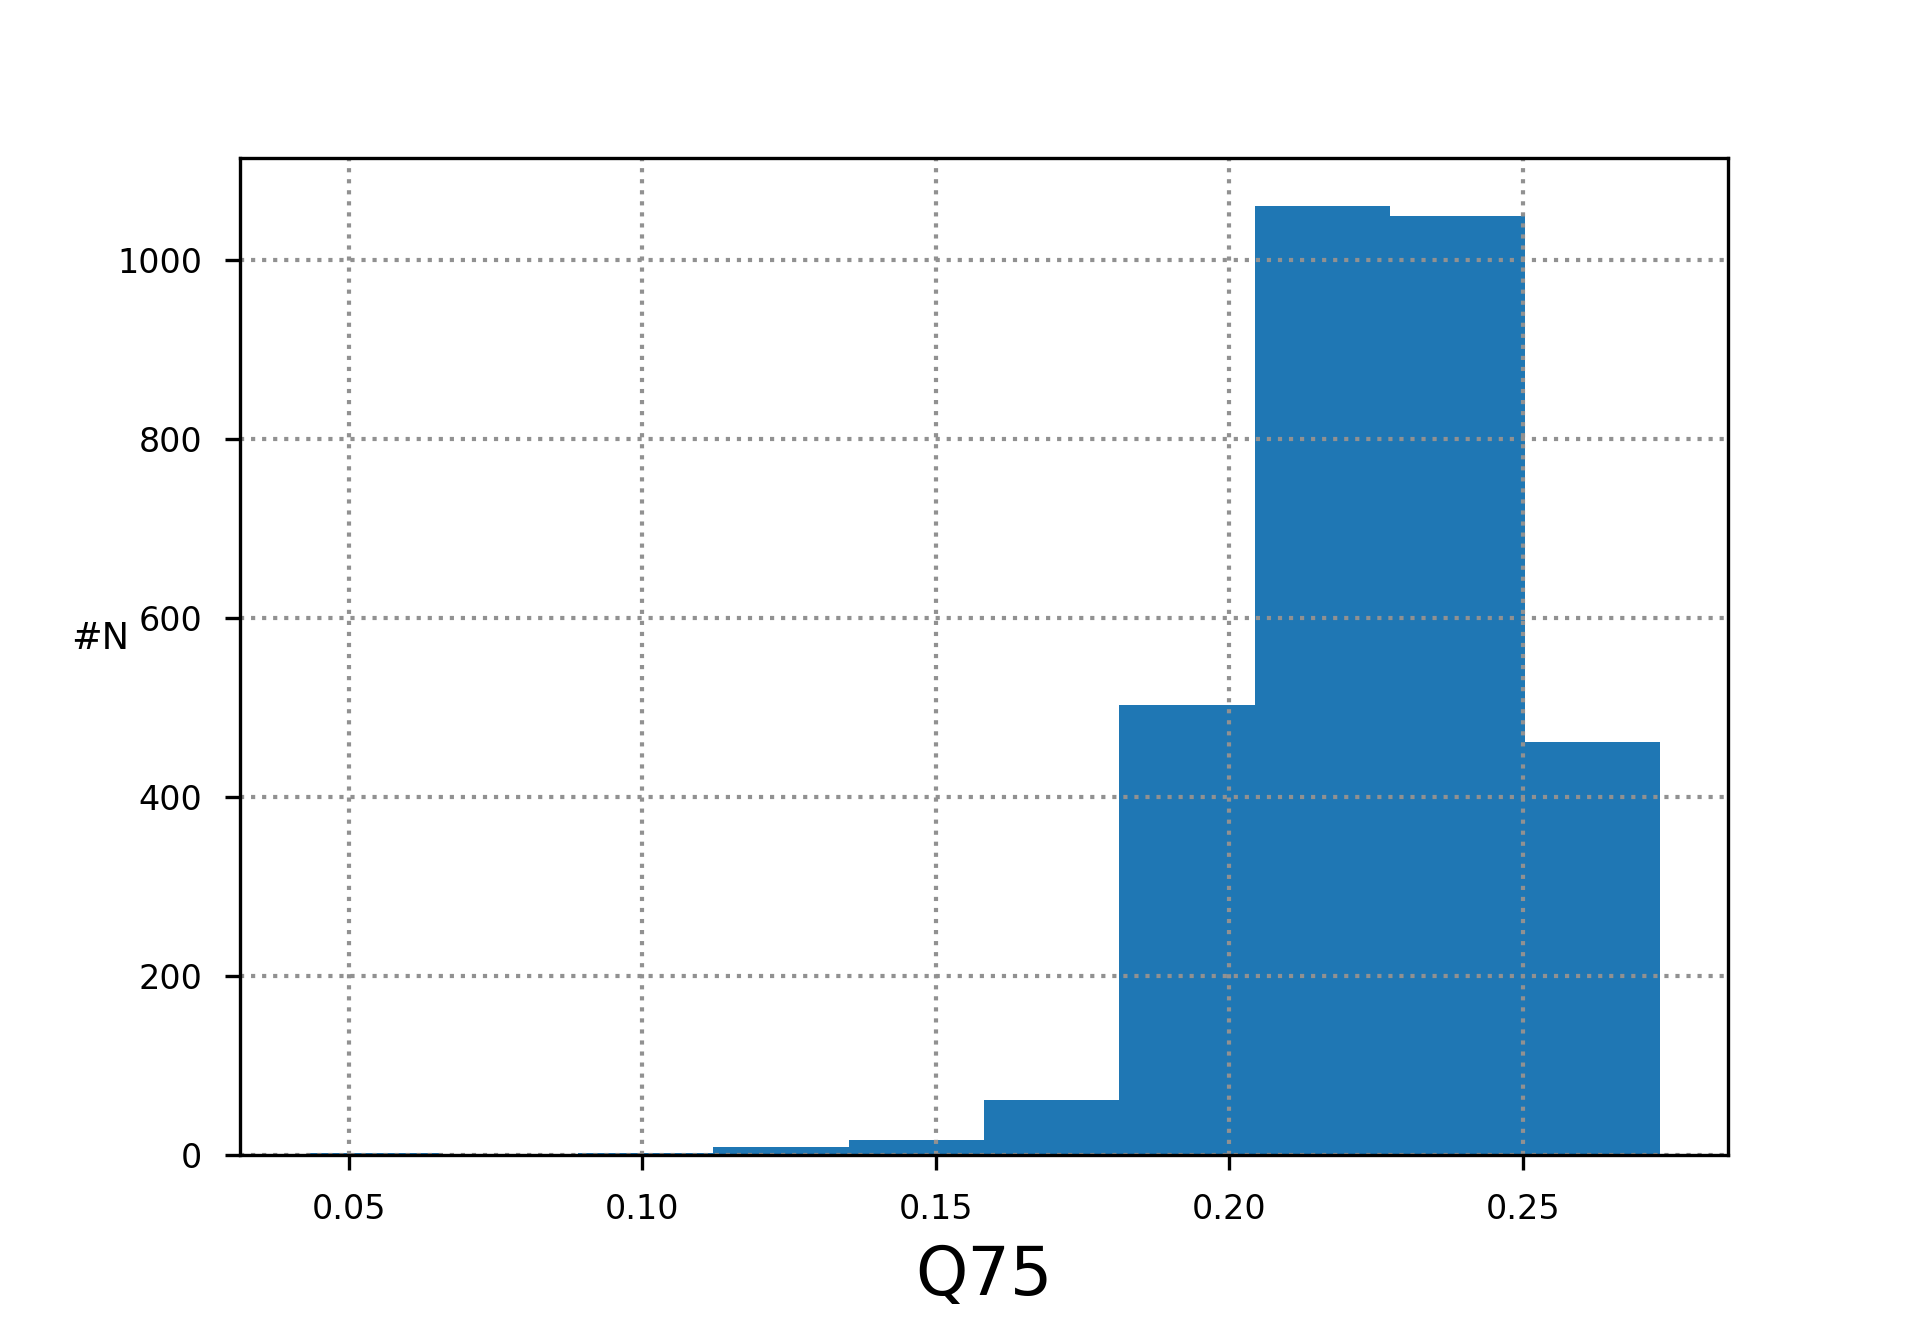
\includegraphics[width=.8\linewidth]{img1/data_histQ75.png}
                \caption{Q75}
            \end{subfigure}
            \begin{subfigure}{.5\textwidth}
                \centering
                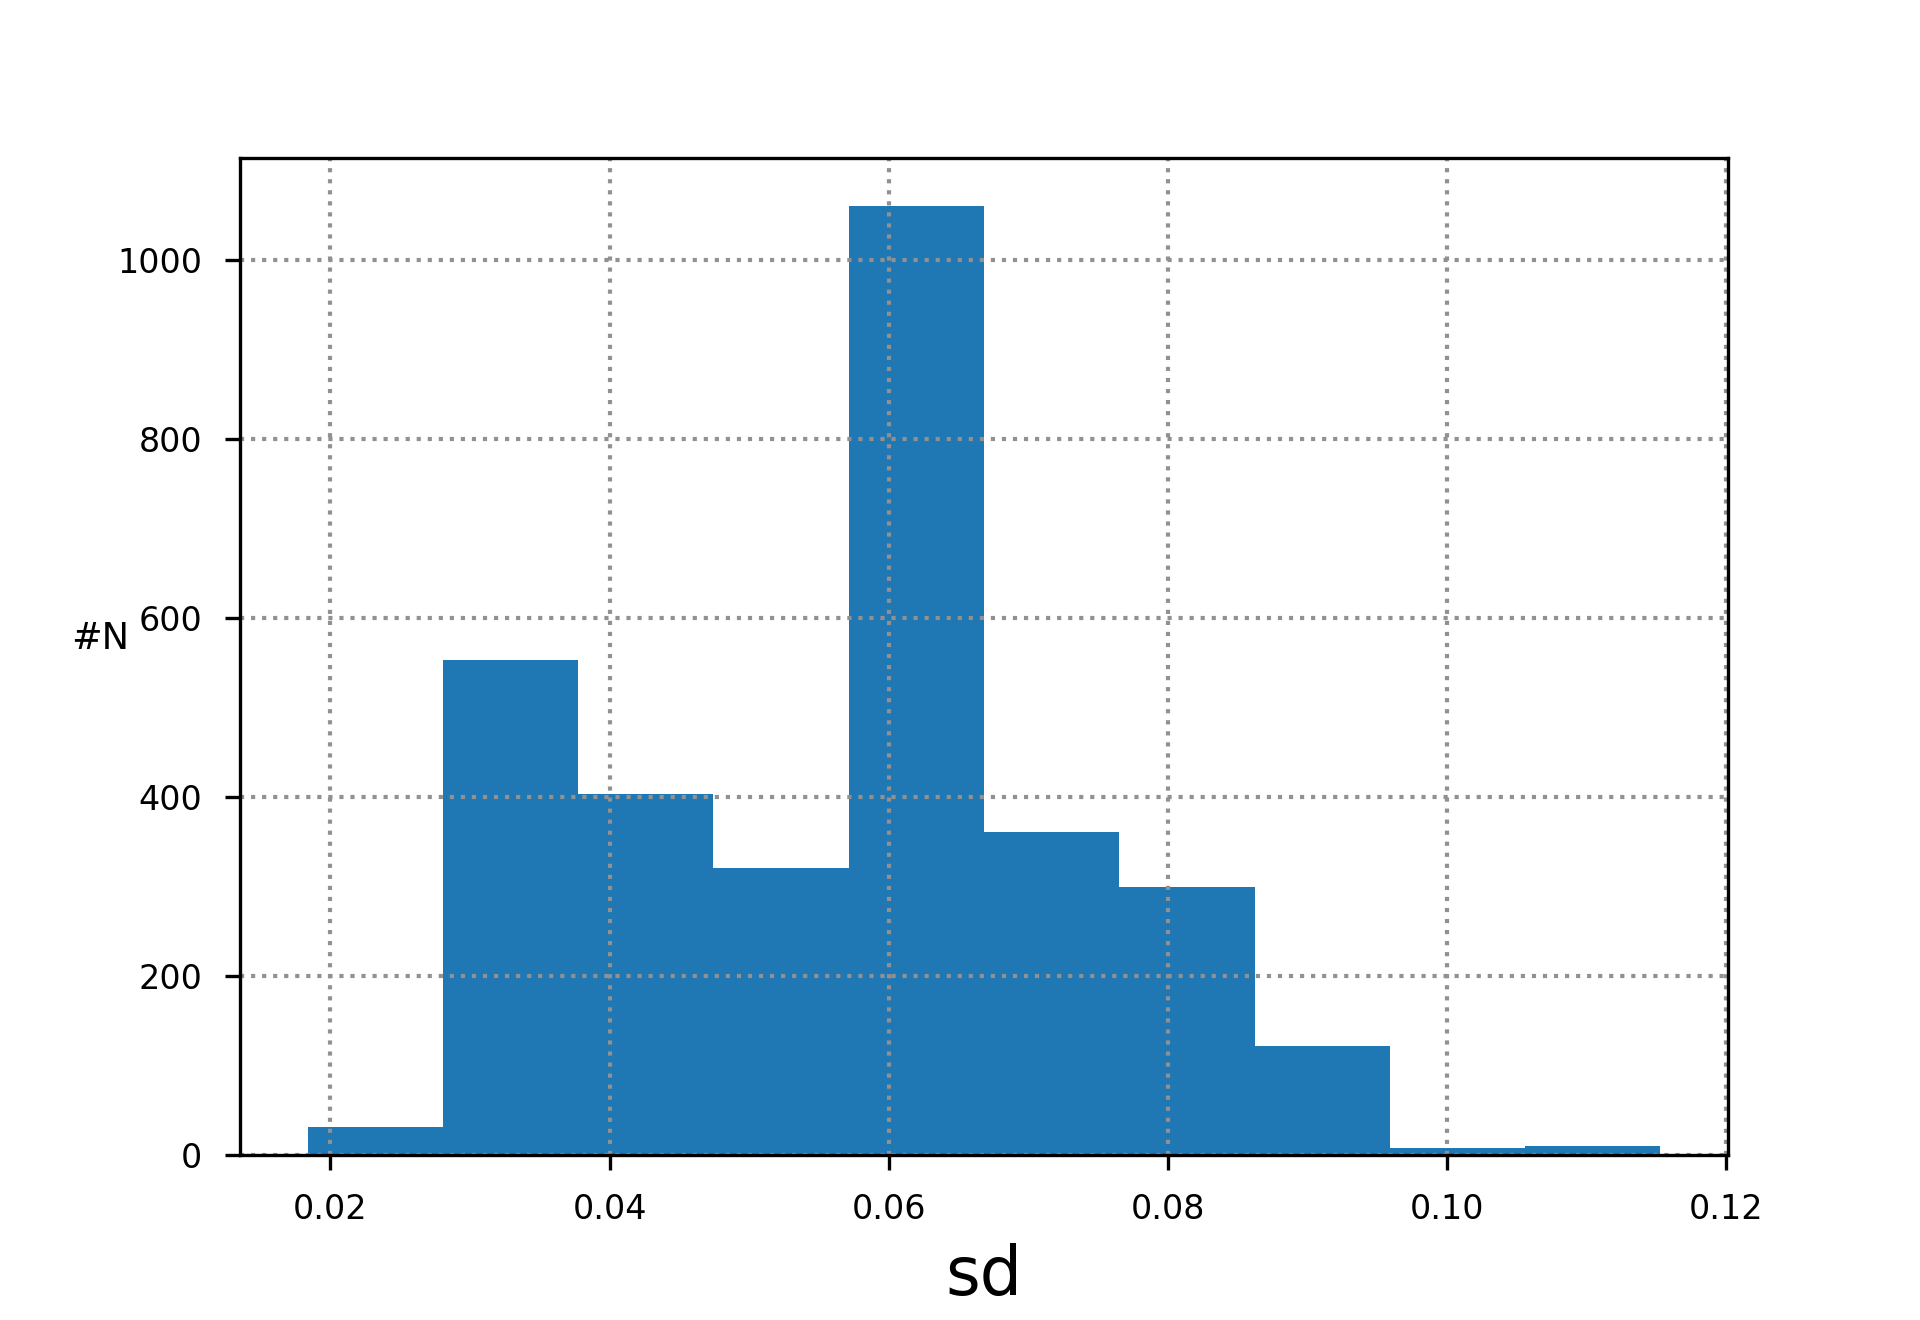
\includegraphics[width=.8\linewidth]{img1/data_histsd.png}
                \caption{sd}
            \end{subfigure}
            \begin{subfigure}{.5\textwidth}
                \centering
                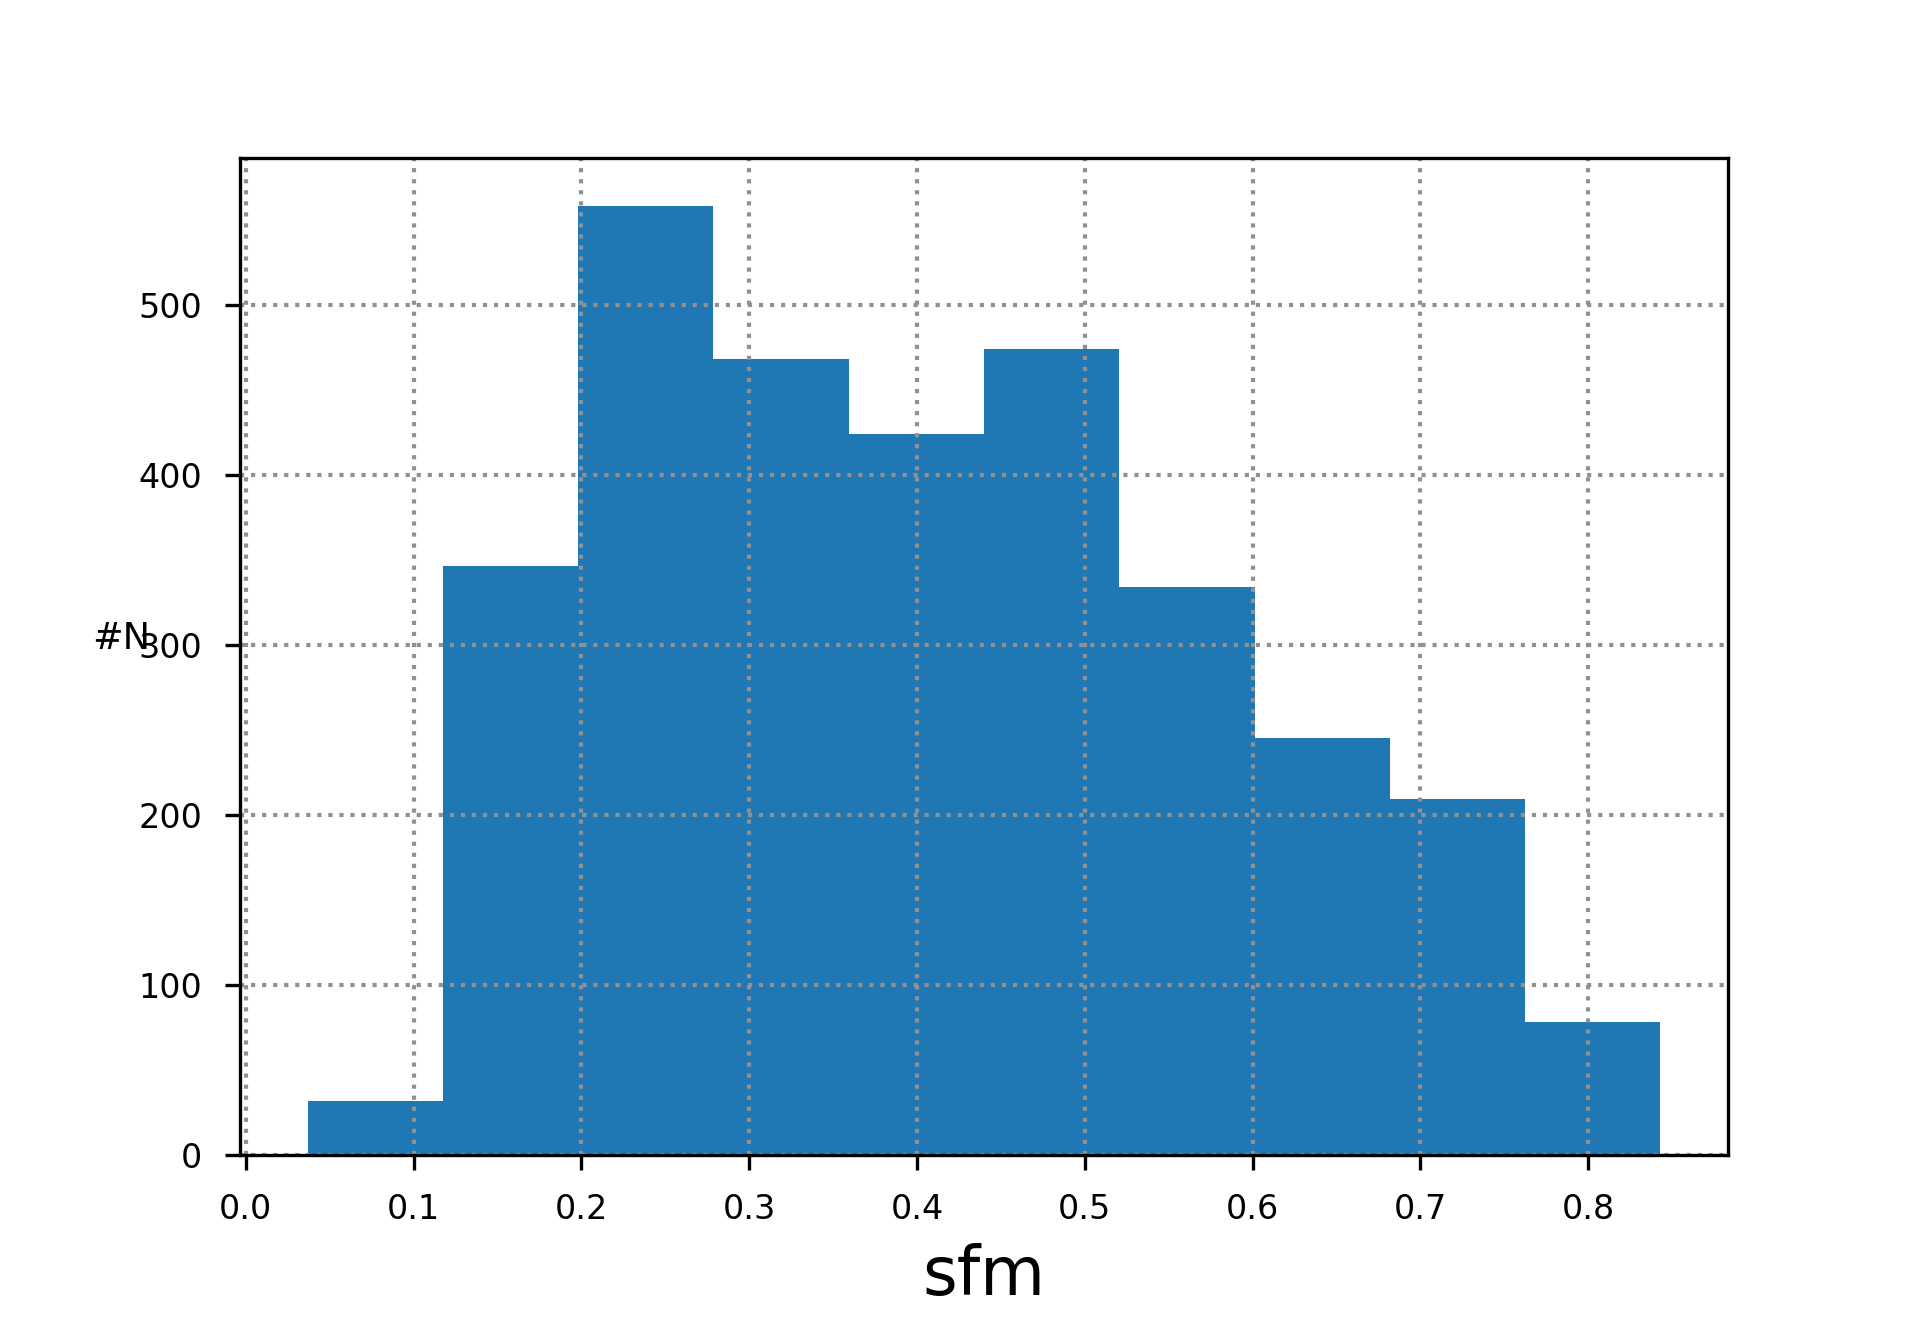
\includegraphics[width=.8\linewidth]{img1/data_histsfm.png}
                \caption{sfm}
            \end{subfigure}
        \caption{Classificação binária: Histograma dos atributos (2)}
        \label{fig:a_hist_2}
        \end{figure}
        \begin{figure}[H]
            \begin{subfigure}{.5\textwidth}
                \centering
                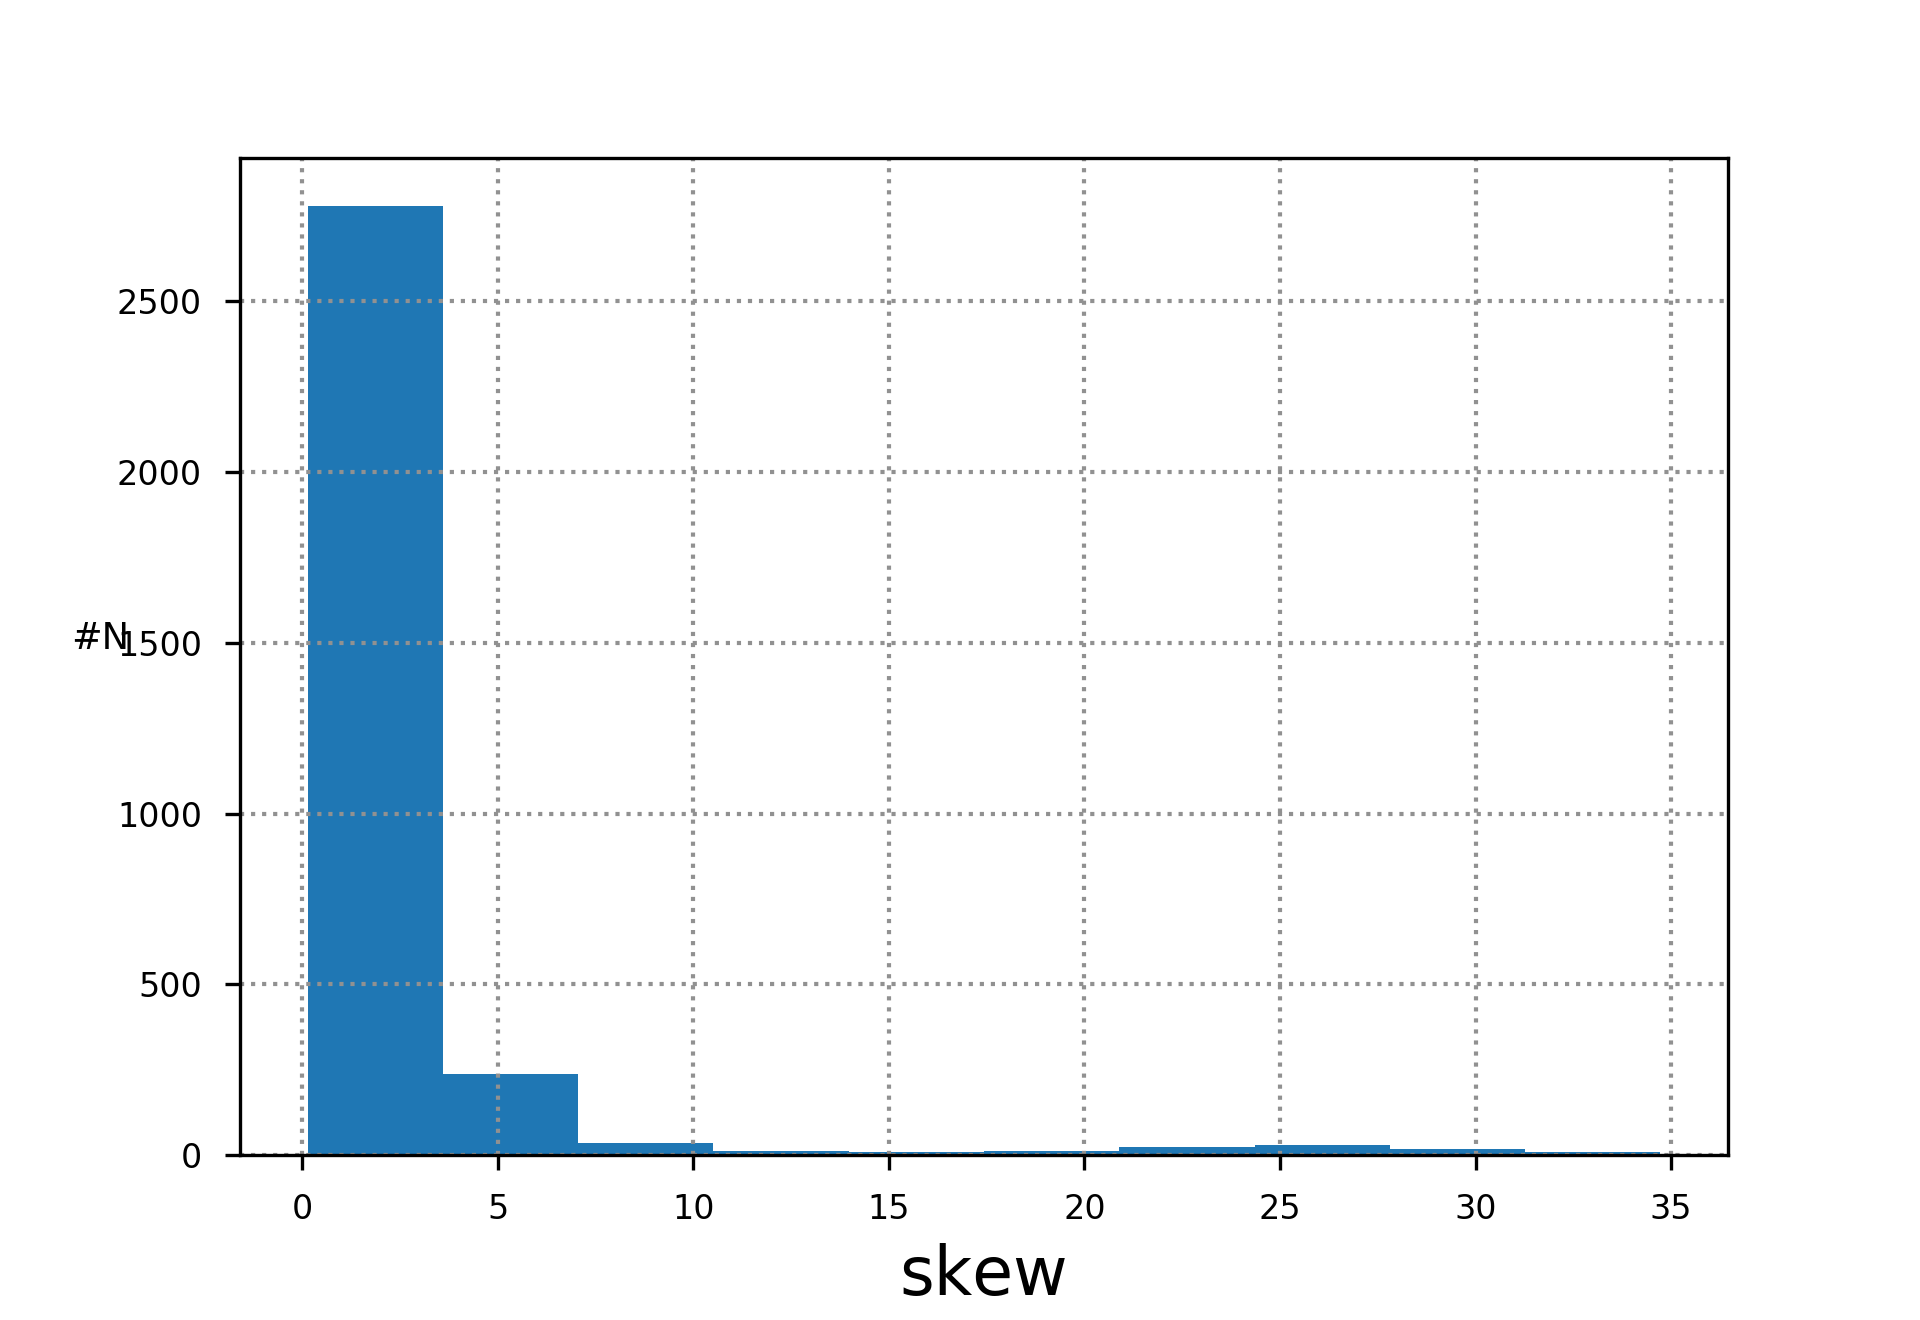
\includegraphics[width=.8\linewidth]{img1/data_histskew.png}
                \caption{skew}
            \end{subfigure}
            \begin{subfigure}{.5\textwidth}
                \centering
                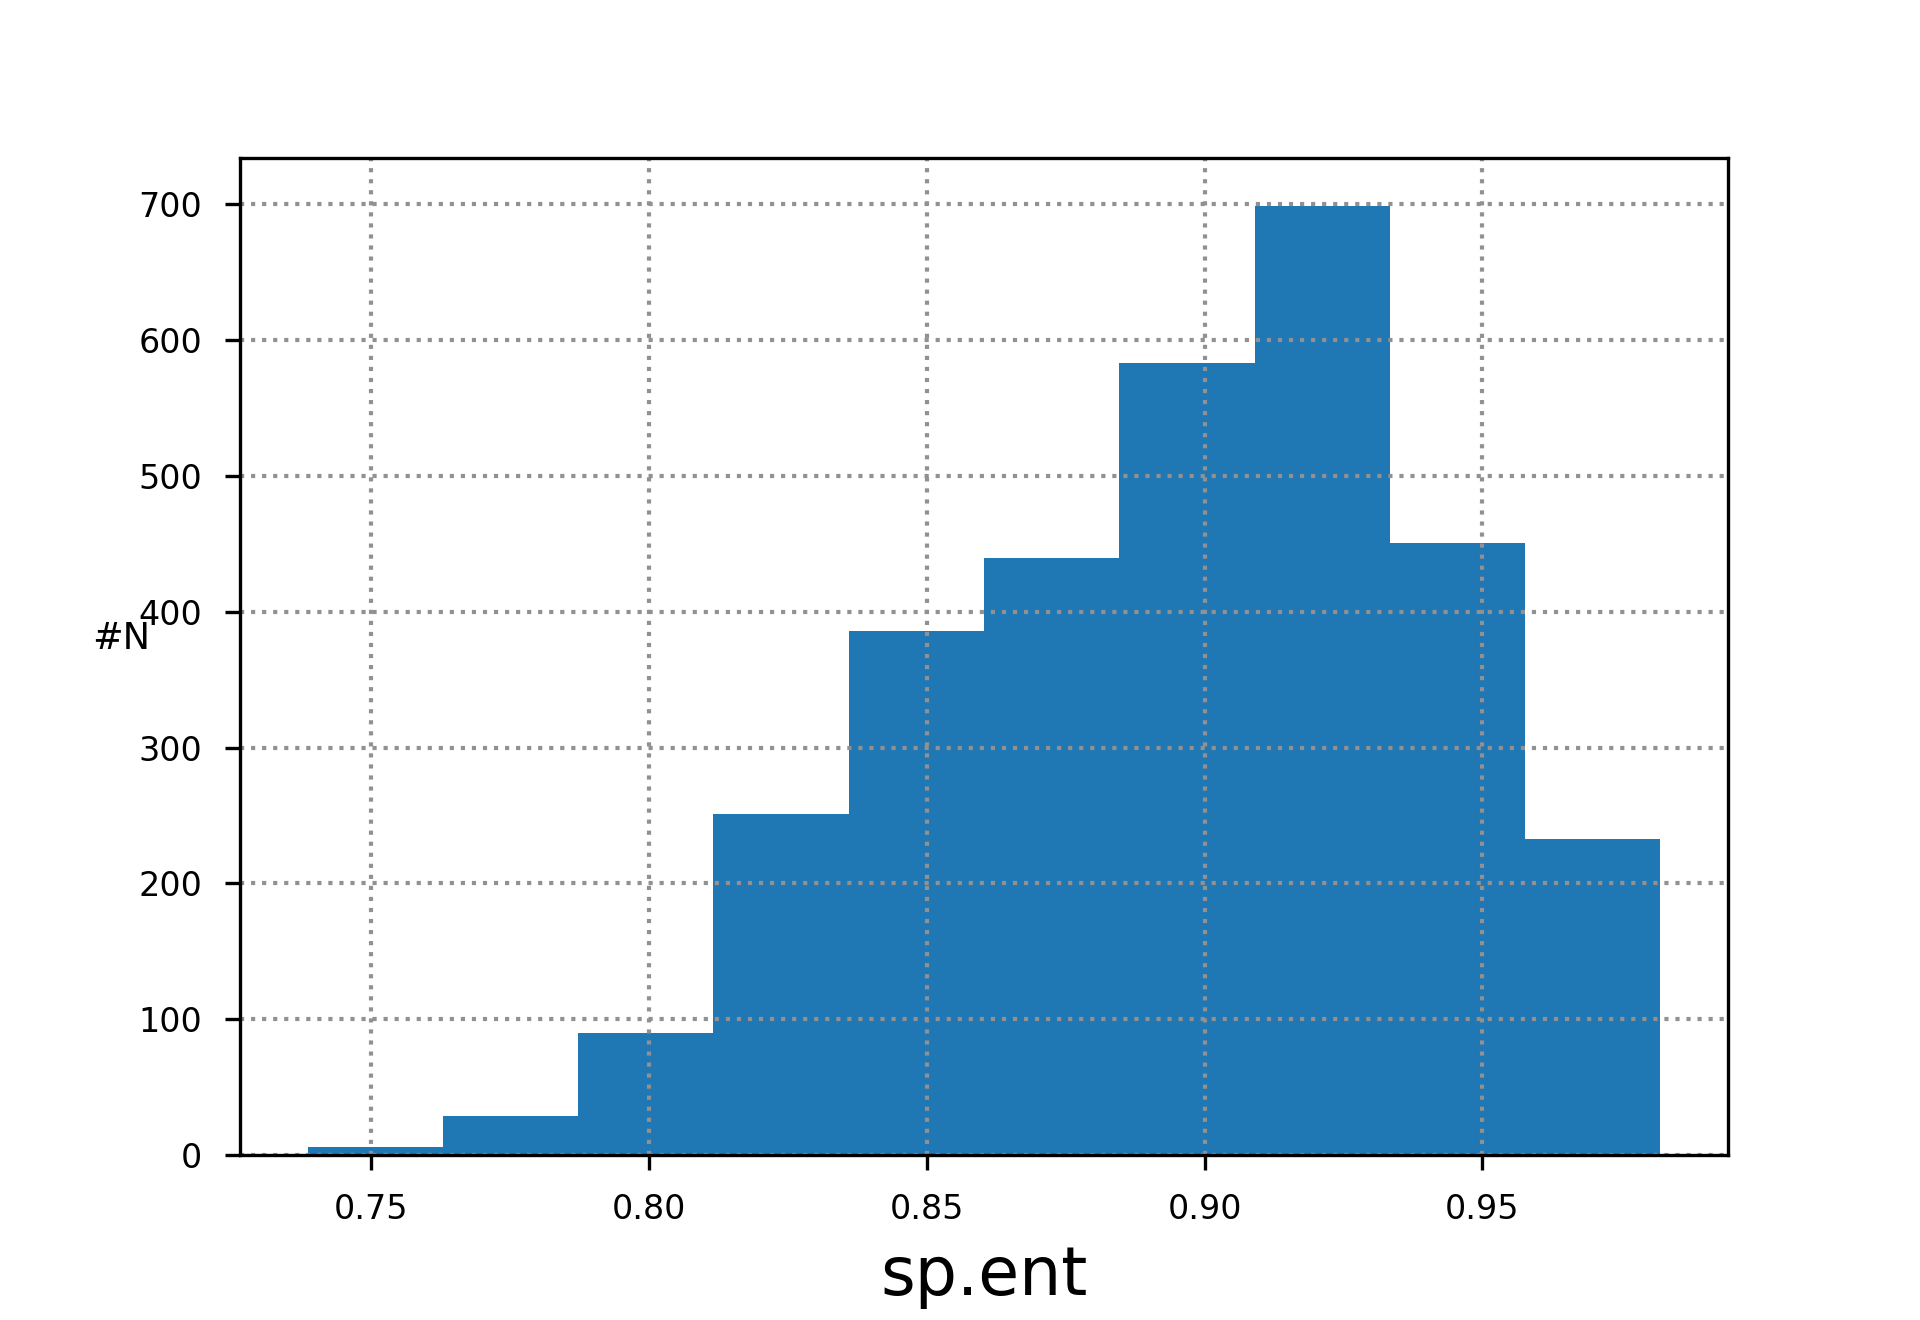
\includegraphics[width=.8\linewidth]{img1/data_histsp_ent.png}
                \caption{histsp.ent}
            \end{subfigure}
            \begin{subfigure}{.5\textwidth}
                \centering
                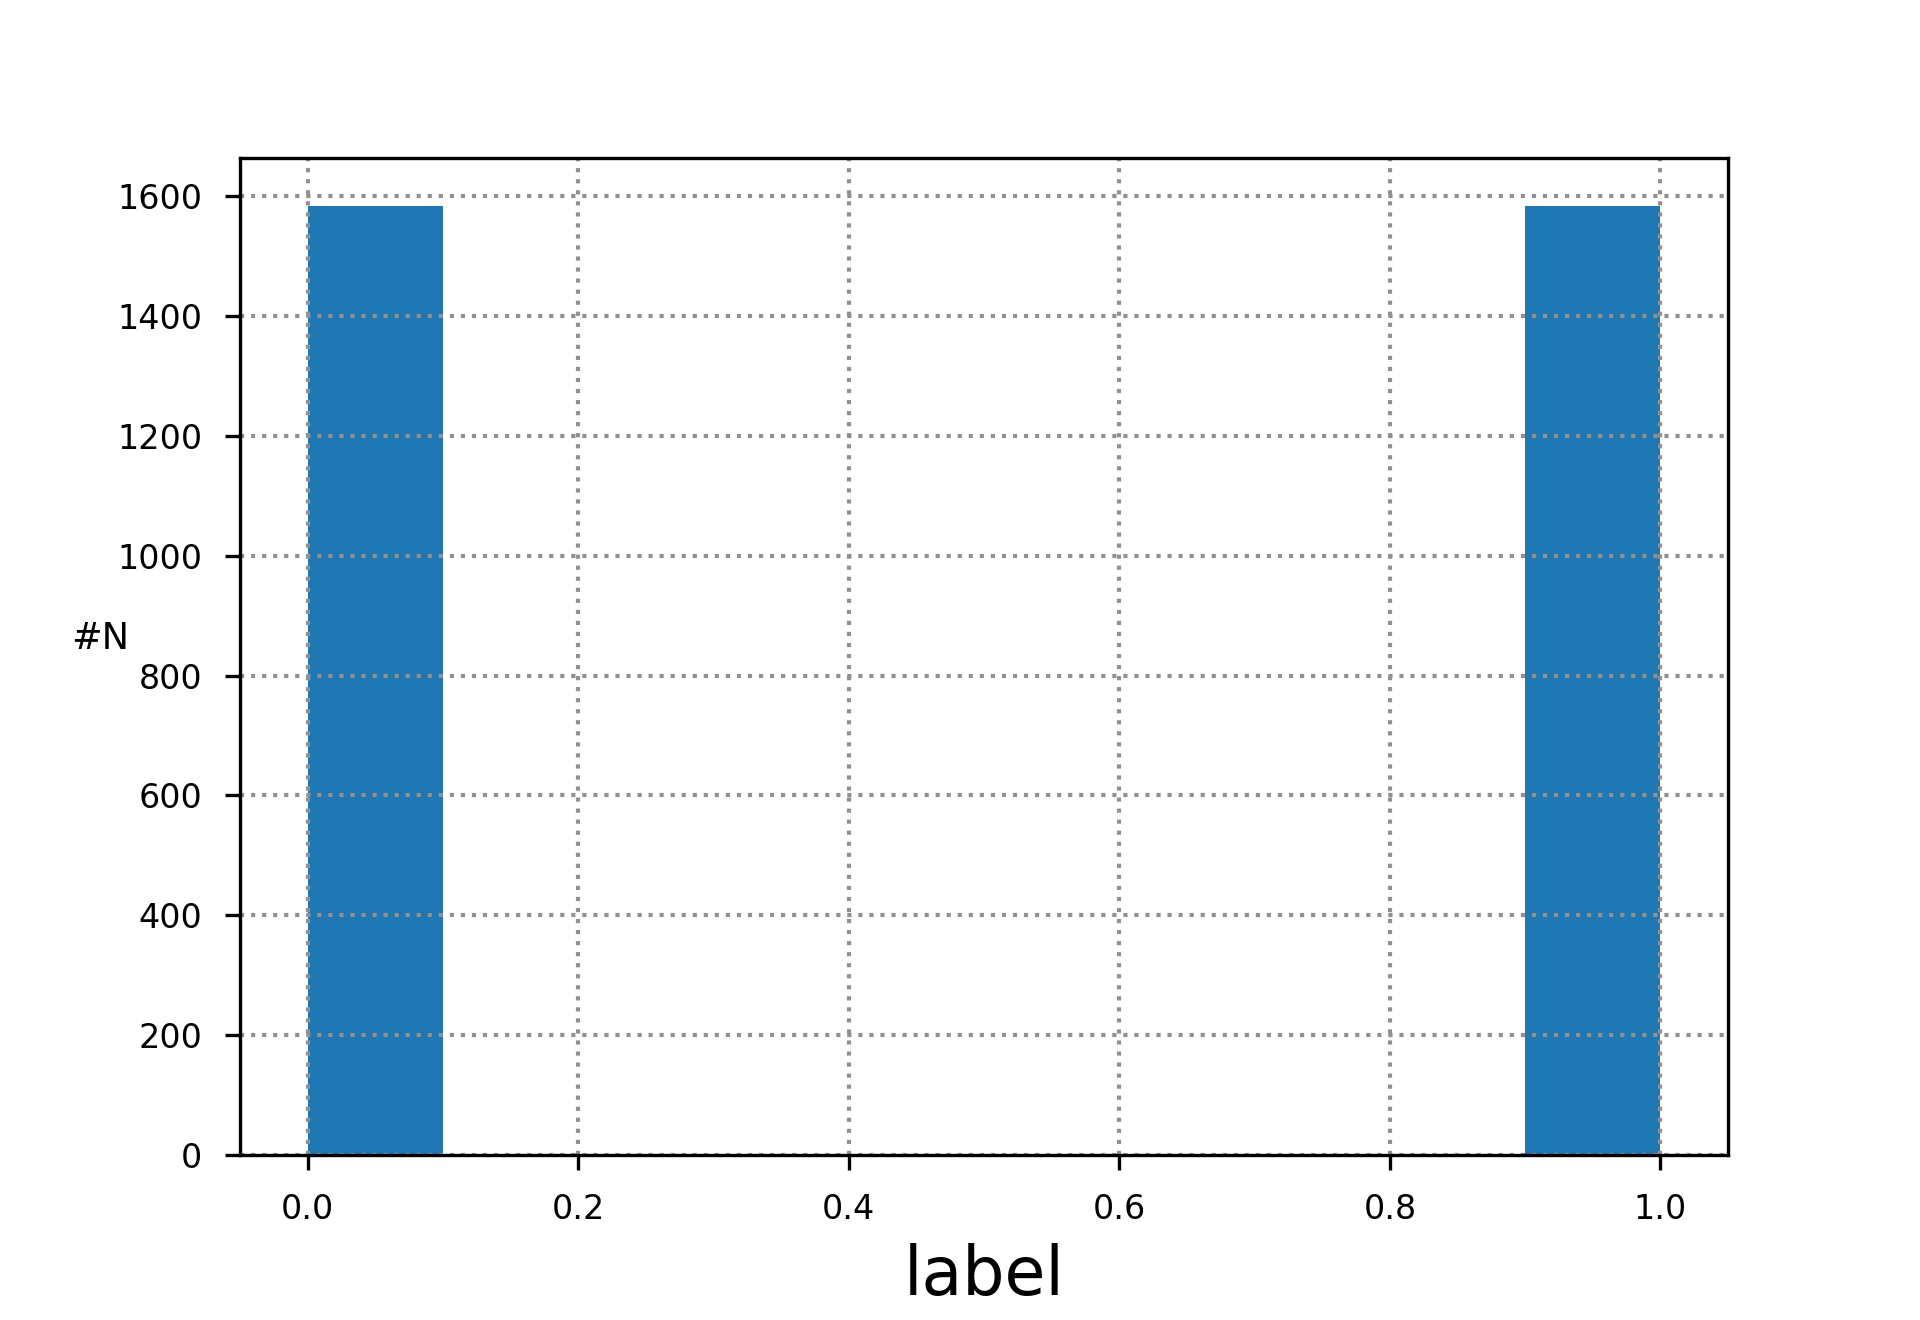
\includegraphics[width=.8\linewidth]{img1/data_histlabel.png}
                \caption{label}
            \end{subfigure}
        \caption{Classificação binária: Histograma dos atributos (3)}
        \label{fig:a_hist_3}
        \end{figure}

        \begin{figure}[H]
            \centering
            \includegraphics[width=.8\linewidth]{img1/data_corr.png}
            \caption{Classificação binária: Mapa de calor da correlaçao dos atributos}
            \label{fig:a_corr_heat}
        \end{figure}
        \begin{figure}[H]
            \centering
            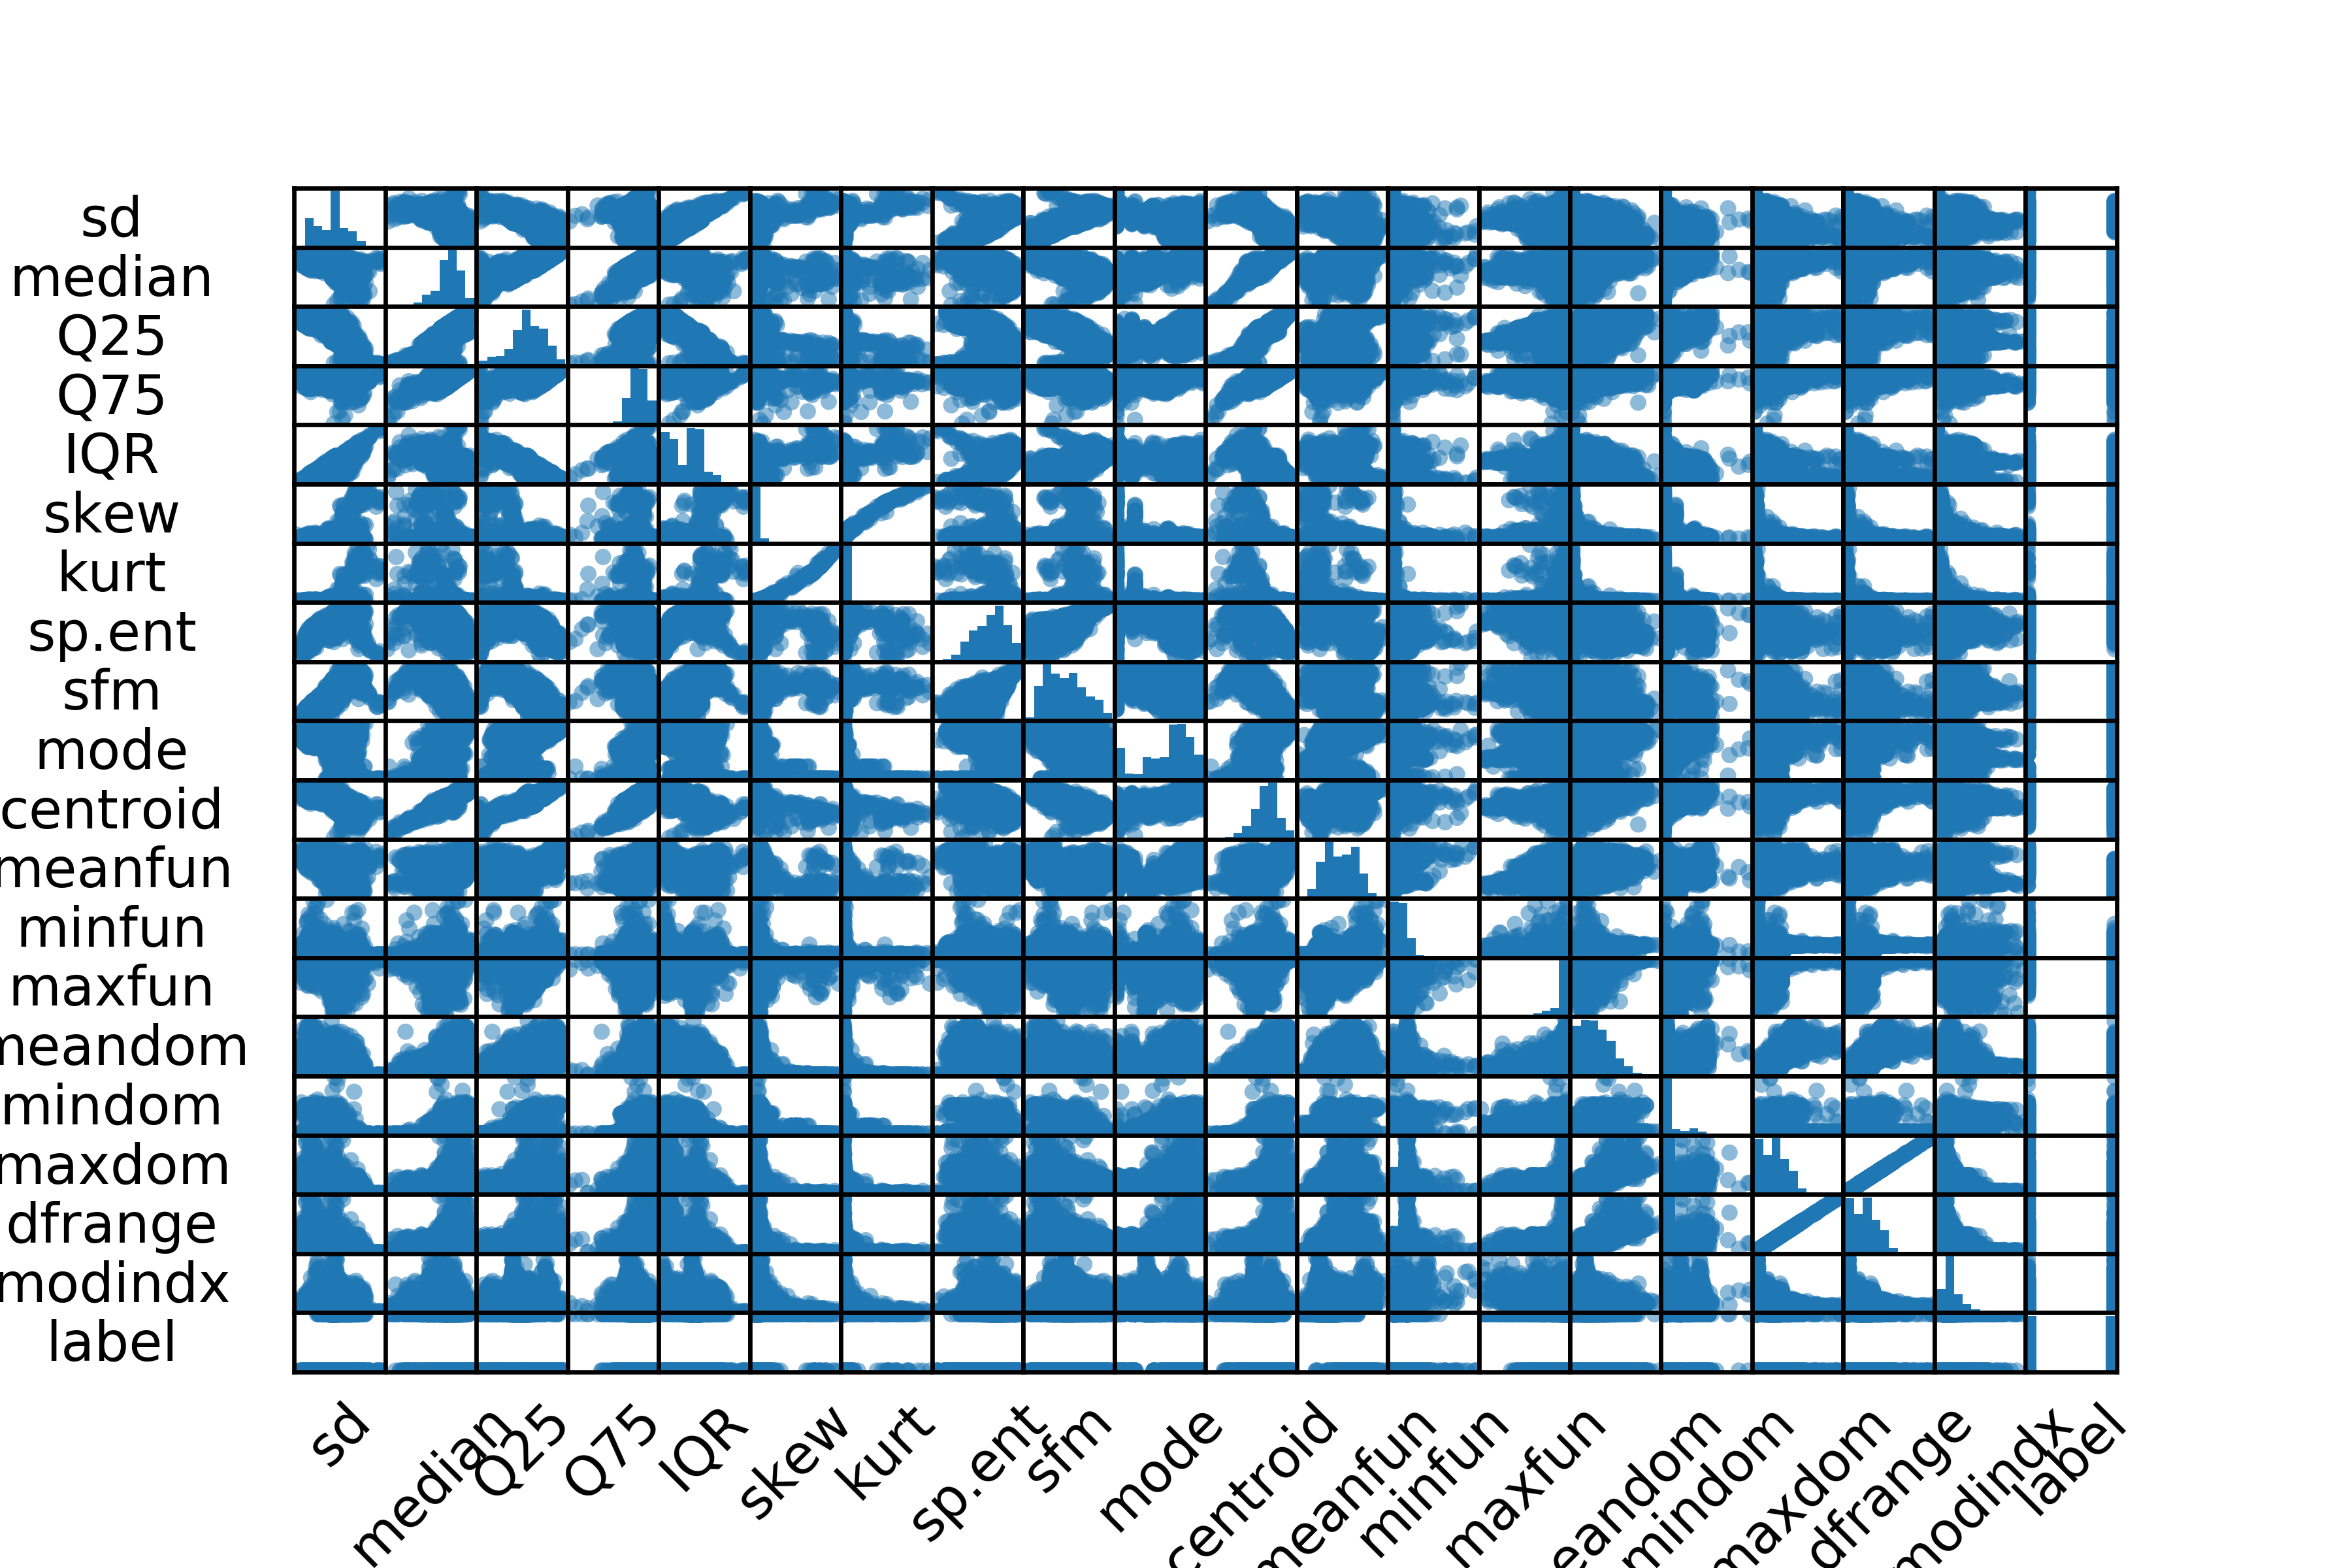
\includegraphics[width=\textwidth]{img1/data_corr_scatter.png}
            \caption{Classificação binária: Correlação dos atributos em gráfico de dispersão }
            \label{fig:a_corr_scatter}
        \end{figure}
    \subsection[]{b) Curva ROC e $F_1$-medida}
        É utilizado o método \textit{Z-score} para normalização dos dados. Tal método foi escolhido
        pois favorece o progresso de algoritmos baseados no gradiente descendente, uma vez que deixa as curvas de nível
        da superfície de erro mais circulares.

        O processo de treinamento tem como critério de parada a variação da função de custo. Quando
        o decréscimo por década do custo for inferior a $10^{-8}$ é terminado o processo de treinamento.

        Parâmetros de treinamento:
        \begin{align*}
            \eta&=10^{-2} \\
            tol&=10^{-8}
        \end{align*}
        sendo $\eta$ a taxa de aprendizagem e $tol$ o limiar para o término do treinamento.
        \begin{figure}[H]
            \centering
            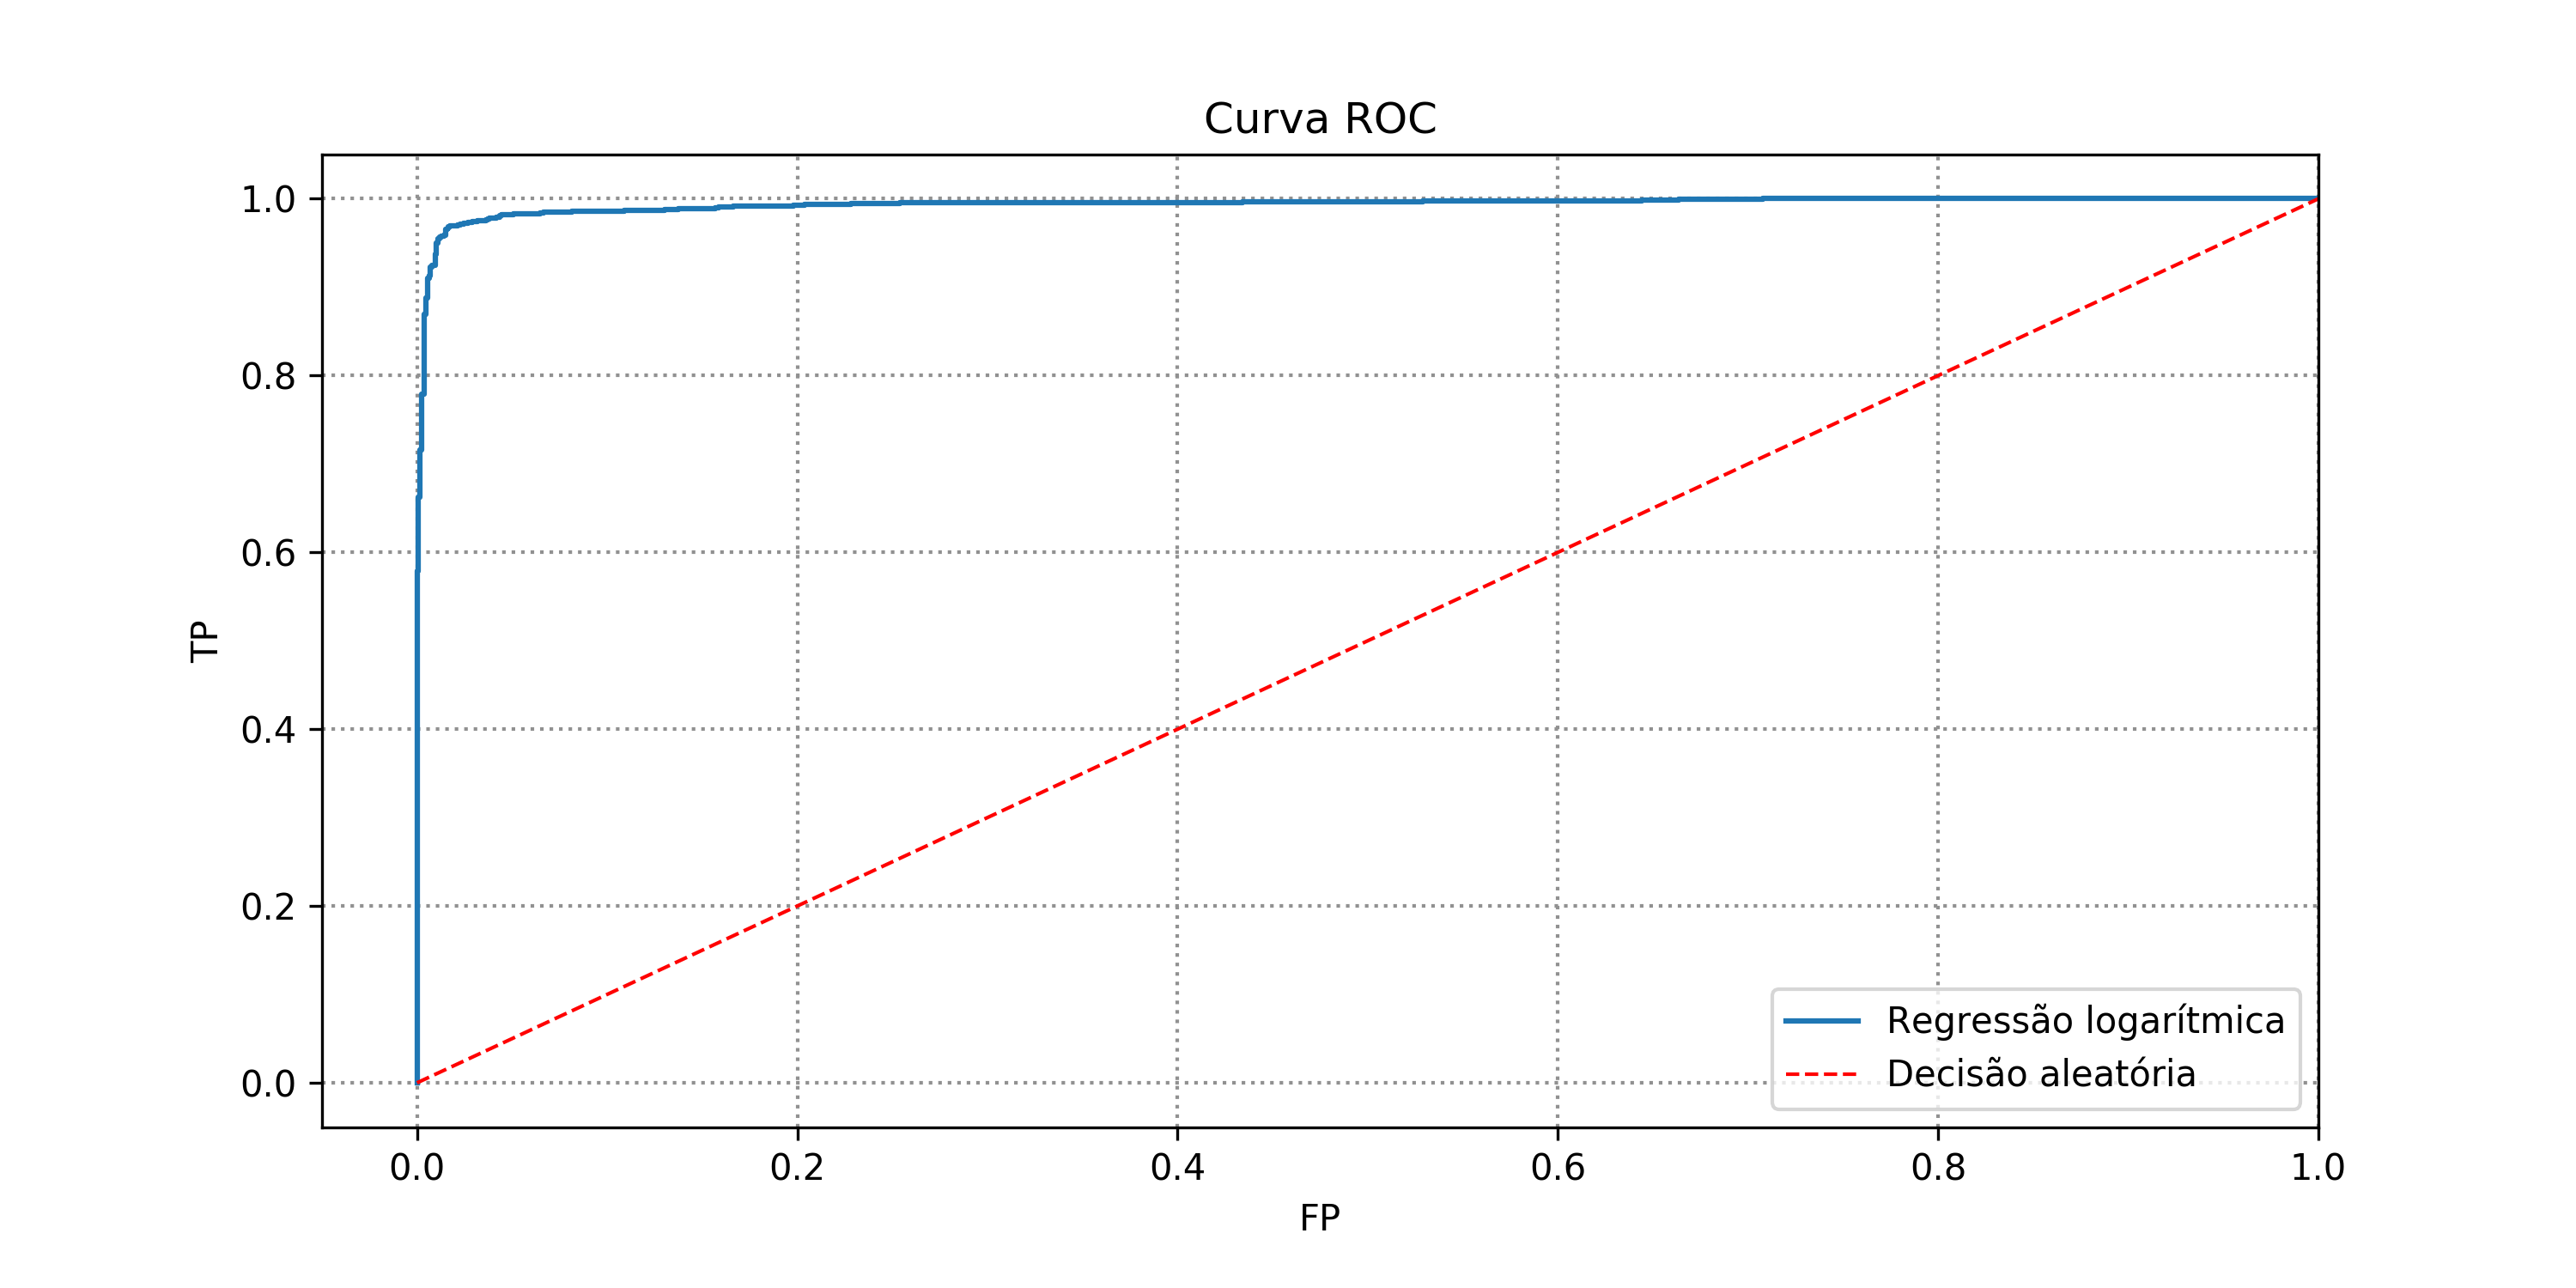
\includegraphics[width=\textwidth]{img1/roc.png}
            \caption{Classificação binária: Curva ROC relativa aos dados de Teste}
            \label{fig:a_roc}
        \end{figure}
        \begin{figure}[H]
            \centering
            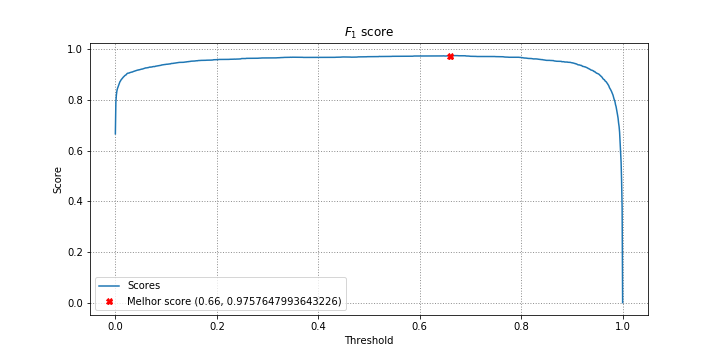
\includegraphics[width=\textwidth]{img1/f1_score.png}
            \caption{Classificação binária: $F_1$-medida relativa aos dados de Teste}
            \label{fig:a_fi_score}
        \end{figure}
    
    \subsection[]{c) Melhor \textit{threshold}, matriz de confusão e acurácia}
    Para a escolha do valor de \textit{threshold} será utilizada a $F_1$-medida, de forma que
    o \textit{recall} e precisão do classificador tenham a mesma importância.

    Conforme apresentado na figura \prettyref{fig:a_fi_score}, o ponto de máxima $F_1$-medida é
    obtido com:
    \begin{align*}
        \textit{threshold}&=0.663 \\
        F_1-medida&\approx0.9757
    \end{align*}
    Utilizando o limiar de máxima $F_1$-medida, a classificação do \textit{dataset} de testes é 
    apresentada conforme a matriz de confusão:
    \begin{table}[H]
        \begin{tabular}{ccccc}
        &  &  & \multicolumn{2}{c}{\textbf{Classe Estimada}} \\
        &  &  & Feminino & Masculino\\
        &  &  & + & - \\ \cline{4-5} 
        \textbf{Classe} & Feminino & \multicolumn{1}{c|}{+} & \multicolumn{1}{c|}{1227} & \multicolumn{1}{c|}{40} \\ \cline{4-5} 
        \textbf{Verdadeira} & Masculino & \multicolumn{1}{c|}{-} & \multicolumn{1}{c|}{21} & \multicolumn{1}{c|}{1246} \\ \cline{4-5} 
        \end{tabular}
    \end{table}
    O classificador apresenta acurácia (acc), precisão (prec) e \textit{recall} de:
    \begin{align*}
        acc & \approx0.9759 \\
        prec & \approx0.9832 \\
        recall & \approx0.9684
    \end{align*}

\end{document}